\documentclass{report}
% Comment the following line to NOT allow the usage of umlauts


\usepackage[utf8]{inputenc}
\usepackage[left=3.5cm,right=3.5cm,top=4cm,bottom=4cm]{geometry}
\usepackage[francais]{babel}
\usepackage{listings}

\usepackage{xcolor}
\usepackage{graphicx, wrapfig, subcaption, setspace, booktabs}
\frenchbsetup{StandardLists=true} % à inclure si on utilise \usepackage[french]{babel}
\usepackage{enumitem}
\usepackage{textcomp}
%\pagestyle{plain}
\usepackage{fancyhdr}



\renewcommand{\headrulewidth}{0.4pt}
\pagestyle{fancy}

\definecolor{listinggray}{gray}{0.9}
\definecolor{lbcolor}{rgb}{0.9,0.9,0.9}
\definecolor{darkWhite}{rgb}{0.94,0.94,0.94}
\lstset{
aboveskip=3mm,
belowskip=3mm,
backgroundcolor=\color{darkWhite},
basicstyle=\footnotesize,
breakatwhitespace=false,
breaklines=true,
captionpos=b,
commentstyle=\color{red},
deletekeywords={...},
escapeinside={\%*}{*)},
extendedchars=true,
framexleftmargin=16pt,
framextopmargin=3pt,
framexbottommargin=6pt,
frame=tb,
keepspaces=true,
keywordstyle=\color{blue},
language={[Sharp]C},
literate=
{²}{{\textsuperscript{2}}}1
{⁴}{{\textsuperscript{4}}}1
{⁶}{{\textsuperscript{6}}}1
{⁸}{{\textsuperscript{8}}}1
{€}{{\euro{}}}1
{é}{{\'e}}1
{è}{{\`{e}}}1
{ê}{{\^{e}}}1
{ë}{{\¨{e}}}1
{É}{{\'{E}}}1
{Ê}{{\^{E}}}1
{û}{{\^{u}}}1
{ù}{{\`{u}}}1
{â}{{\^{a}}}1
{à}{{\`{a}}}1
{á}{{\'{a}}}1
{ã}{{\~{a}}}1
{Á}{{\'{A}}}1
{Â}{{\^{A}}}1
{Ã}{{\~{A}}}1
{ç}{{\c{c}}}1
{Ç}{{\c{C}}}1
{õ}{{\~{o}}}1
{ó}{{\'{o}}}1
{ô}{{\^{o}}}1
{Õ}{{\~{O}}}1
{Ó}{{\'{O}}}1
{Ô}{{\^{O}}}1
{î}{{\^{i}}}1
{Î}{{\^{I}}}1
{í}{{\'{i}}}1
{Í}{{\~{Í}}}1,
morekeywords={*,...},
numbers=left,
numbersep=10pt,
numberstyle=\tiny\color{black},
%rulecolor=\color{black},
showspaces=false,
showstringspaces=false,
showtabs=false,
stepnumber=1,
stringstyle=\color{gray},
tabsize=4,
title=\lstname,
}


\newcommand{\HRule}[1]{\rule{\linewidth}{#1}}
\onehalfspacing

%-------------------------------------------------------------------------------
% HEADER & FOOTER
%-------------------------------------------------------------------------------
\pagestyle{plain}
\fancyhf{}
\setlength\headheight{15pt}
\fancyhead[L]{Metabot : Un jeu multi-agent générique}
\fancyhead[C]{TER}
\fancyhead[R]{Université de Montpellier}
\fancyfoot[R]{\today}

%-------------------------------------------------------------------------------
% TITLE PAGE
%-------------------------------------------------------------------------------

\begin{document}
\pagenumbering{Roman}
\title{\normalsize \textsc{Rapport de TER}
		\\ [1.5cm]
		\HRule{0.5pt} \\
		\LARGE \textbf{\uppercase{Metabot\\Un jeu multi-agent générique}}\\\HRule{0.5pt} \\}

\date{}

\author{\\[0.5cm] \textit{Equipe Interface Graphique}\\
		\textsc{Fumey} David \\
	\textsc{Dorey} Benoit \\[0.15cm] \\
	\textit{Equipe Moteur} \\	
	\textsc{BenLamine} Mehdi \\
	\textsc{Teixeira-Ricci} Maxime \\ [0.15cm] \\
	\textit{Supervisé par} M. \textsc{Ferber} Jacques\\ [2.5cm]\\
	Université Montpellier - Master 1 Informatique}

\maketitle


\chapter*{Remerciements}
Nous tenions à remercier notre encadrant M.Ferber, qui nous a suivi et conseillé durant toute la durée de ce projet.\newline
Nous tenions également à créditer les créateurs de certaines icônes et polices faisant partie de notre projet.

\section*{Icônes}
\noindent
New file icon : Creative Stall\newline
Load file icon : Ralf Schmitzer\newline
Save icon : To Uyen\newline
Undo : Michael Kussmaul\newline
Redo : ImageCatalog\newline
Sound Icon : Yaroslav Samoyl\newline
Muted sound icon : Dev Patel\newline
\section*{Polices}
\noindent
Enchanted Land\newline
Dennis Ludlow

\tableofcontents
\newpage
% Create a new 1st level heading
\pagenumbering{arabic}
\part{Présentation du projet}
\chapter{Introduction}
\section{But du projet}
\paragraph{}
L'objectif de ce projet est la réalisation d'un jeu basé sur un modèle multi-agent. L'idée générale du projet est dans la continuité de celui de l'année dernière et sur le même thème. L'outil utilisé est Unity 3D, un moteur de jeu employé dans un grand nombre de réalisations de hautes qualités. Notre projet fonctionne sur Windows et pourrait être porté sur Mac ou encore Android.
Ce projet consiste de réaliser un jeu que l'on peut qualifier de programmeur et de permettre, notamment, à de jeunes personnes de se familiariser avec le monde de la programmation. L'utilisateur pourra donc créer un comportement pour des robots appelés "unités" afin de remplir des objectifs du jeu.
\paragraph{}
\textsc{Metabot} est un projet modeste réalisé à partir du logiciel Unity 3D par un groupe d'étudiants débutants dans l'utilisation de cet outil. Malgré le peu d'expérience dans la création pure de ce genre d'applications, le projet actuel est le fruit d'un travail important et d'une implication entière de toute l'équipe.
Il a donc pour unique prétention de communiquer notre amour du jeu vidéo et de la programmation.

\section{Cahier des charges}

Notre but était de modifier le programme existant afin qu'il devienne plus générique. C'est à dire qu'il ne se limite plus au simple jeu Warbot mais qu'il permette l'implémentation de différents jeux orientées agents facilement. 
Pour cela il fallait donc généraliser la gestion des différentes unités et de leur comportement (action/perception/statistique). De plus, l'ajout d'actions et de moyens de perceptions doit se faire de façon intuitive de même pour les différentes exigences de jeu (règles/conditions de victoire). 

\section{Notion d'agent}
Dans cette section, nous allons développer la notion d'agent dans un système multi-agent.
\subsection{Système multi-agents}
\paragraph{} Un agent dans un système multi-agents est une entité autonome définit par un comportement créer par son auteur. Les agents peuvent aussi interagir avec leur environnement grâce à des perceptions et qui lui permet de lui donner une représentation de ce dernier. 

\begin{figure}[h]
\centering
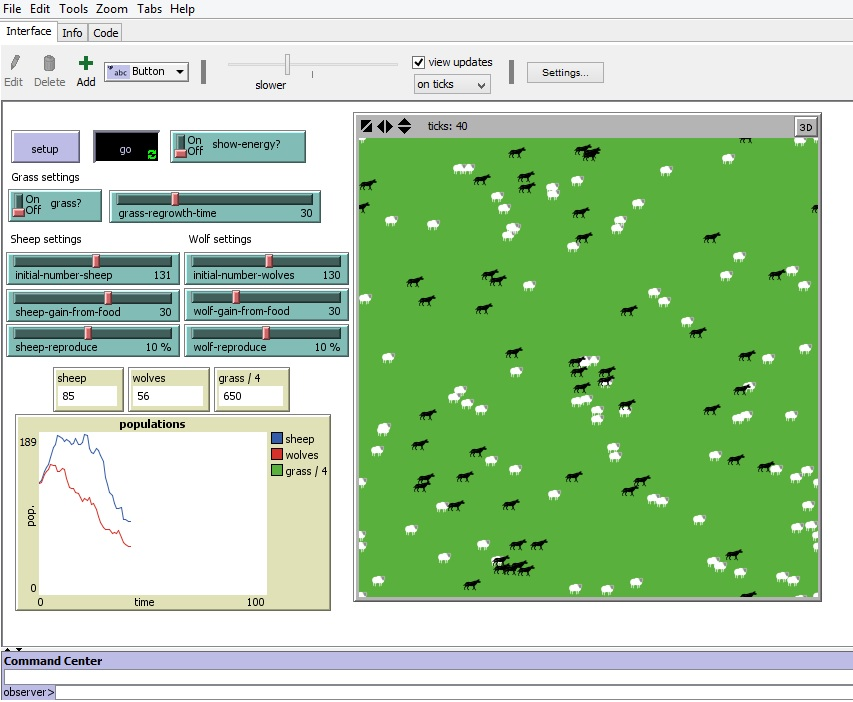
\includegraphics[scale=0.65]{NetLogoImage}
\caption{NetLogo : Un logiciel de simulation multi-agents.}
\end{figure}

\paragraph{L'individualisme au service du collectif.}L’intérêt des agents est l'idée qu'une action individualiste et égoïste permet un comportement collectif d'un ensemble d'agents pour réaliser des actions qu'un individu seul ne pourrais pas accomplir. Pour permettre de réaliser des objectifs de groupe, les individues peuvent communiquer entre eux afin de permettre de déléguer ou de s'unir dans des tâches plus ardues.
\paragraph{Représentation et simulation.}Ce genre de système permet, en créant des comportements d'agents simple, la simulation de société plus complexe. Ainsi, on peut étudier les comportement globales des entités selon ce que l'on veut observer.
\paragraph{Les système-multi agents dans de multiples domaines.} Les systèmes multi-agents sont utilisées dans de nombreux domaines, notamment dans les jeux vidéos et le cinéma. Dans ces domaines, les systèmes multi-agents  sont utilisées pour représenter des mouvement de foules avec des comportement très simples, ou, dans le cas du jeu vidéo, permettre de créer des comportements aux personnages non joueurs pour les rendre plus intéressant pour le joueurs.


\subsection{Représentation dans le projet}

\paragraph{WarBot: Le mode par défaut}
\paragraph{}
\begin{figure}[h]
    \begin{minipage}[c]{.46\linewidth}
        \centering
        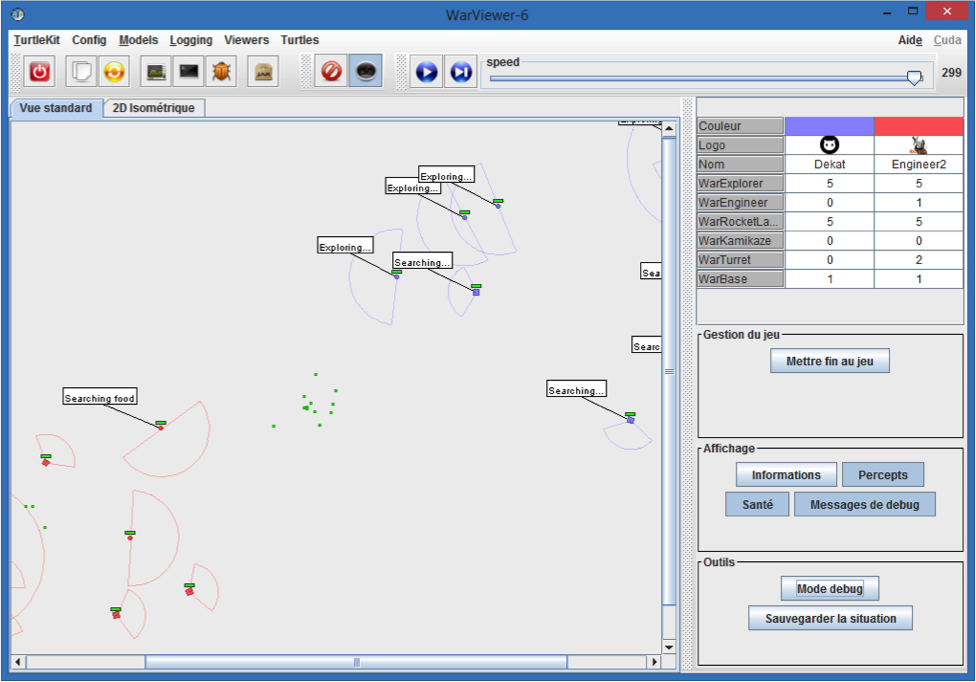
\includegraphics[scale=0.45]{interface-warbot3}
        \caption{WarBot, la version Java.}
    \end{minipage}
    \hfill%
    \begin{minipage}[c]{.46\linewidth}
        \centering
        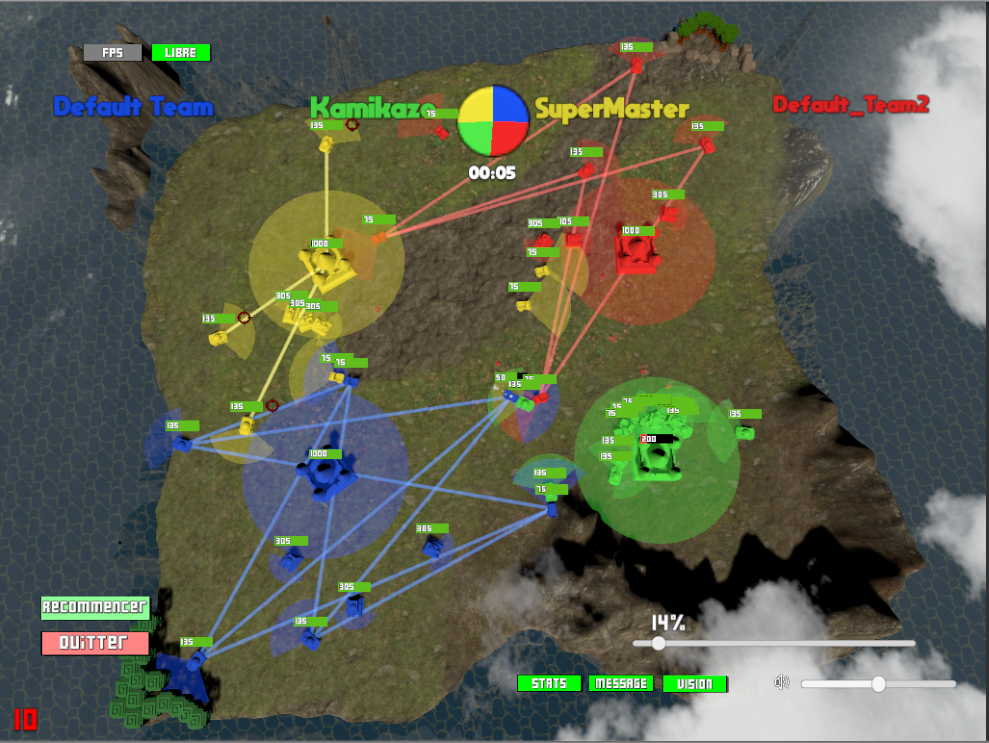
\includegraphics[scale=0.3]{WarbotUnity}
        \caption{WarBot, la version Unity.}
    \end{minipage}
\end{figure}

\subsubsection{Warbot Java en quelques mots}
\paragraph{}Dans WarBot, deux équipes se battent sur un terrain pour les ressources afin de survivre, d'éliminer l'autre équipe et d’être la dernière en vie. Des ressources apparaissent sur la carte et peuvent être converties en unités ou en soin.
\paragraph{}Une équipe est composé d'un ensemble de sept unités :  la WarBase (base), le WarExplorer (explorateur), le WarEngineer (ingénieur), le WarLight (char léger), le WarHeavy (char lourd), le RocketLauncher (lance-missile) et la Turret (tourelle). 
\paragraph{}Le joueur doit programmé le comportement de son équipe, en particulier une architecture de subsomption ou une machine à état finie peuvent être développées dans ce but. 
\paragraph{}Ce programme est utilisé dans le cadre du module de programmation par agents du M1 d'informatique de l'université de Montpellier. Une nouvelle version du moteur de jeu, appelée \textit{Warbot3}, a été l'objet de plusieurs TER.



\newpage
\part{Réalisation du projet}
\newpage

%%%
% PARTIE MOTEUR
%%%
\chapter{Partie Moteur}

\begin{figure}[h]
\centering
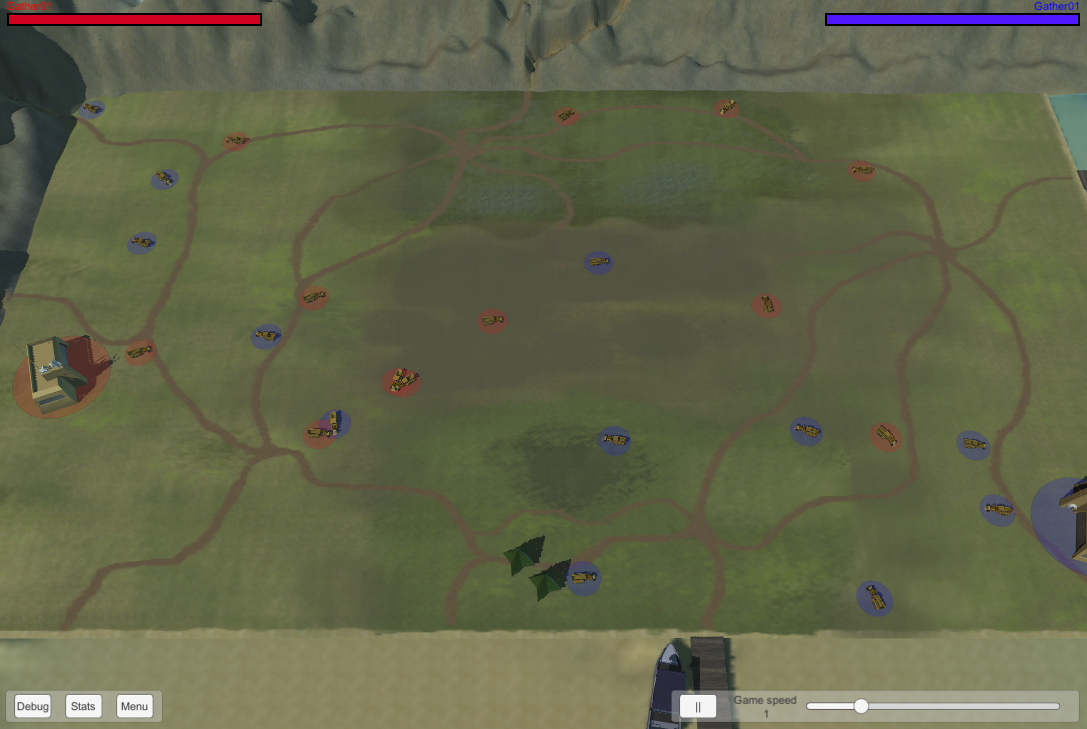
\includegraphics[scale=0.375]{OldWarbotUnityImage}
\caption{L'ancien projet de \textit{Warbot} sous Unity.}
\end{figure}

\section{État de l'art de l'ancien projet.}
 
Pour commencer, attardons nous un moment sur l'ancien projet. L'an dernier, l'objectif premier était de réussir à implémenter le jeu Warbot sous Unity. Le constat que l'on peut faire de ce logiciel est que l'équipe précédente à montrer qu'il est possible de créer un jeu multi-agent en se servant de ce moteur de jeu.
En effet, le Warbot Unity d'origine doté de son menu principal, son interface de paramétrage de partie et sa scène de jeu a déjà pas mal d'atout visuels, mais il n'est pas exempt de bugs et reste assez limité.
Dans cette version, il est donc possible de lancer une partie à deux joueurs uniquement, de régler le nombre de ressources créées par minutes ainsi que la quantité d'unités souhaitées de chacun des cinq types disponibles : WarBase, WarExplorer, WarHeavy, WarEngineer et WarTurret. Une seule carte de jeu rectangulaire et sans obstacles est présente. 

\paragraph{}Durant une partie, le joueur peut effectuer plusieurs actions :
\begin{itemize}
\item Activer l'affichage d'un tableau indiquant le nombre de chaque unités détenue par les deux équipes.
\item Modifier la vitesse du jeu (accélération / ralentissement / pause).
\item Créer une unité pour l'une des deux équipes mais le nombre d'unités est mis à jour pour la mauvaise équipe.
\item Supprimer une unité mais le nombre d'unités n'est pas mis à jour.
\item Déplacer une unité.
\item Activer l'affichage des statistiques d'une unité (vie, ressources détenues, type, ...).
\item Activer l'affichage du suivi visuel des envoies de messages entre unités.
\item Activer l'affichage du groupe auquel appartient une unité mais l'utilisation de groupe dans les comportements n'est pas fonctionnelle.
\item Activer l'affichage de la barre de vie d'une unité.
\item Activer l'affichage de la barre de ressource d'une unité.
\end{itemize}
%A voir si a compléter

\section{Refonte du noyau.}
\paragraph{}L'ancien projet est une adaptation du jeu Warbot crée en Java en utilisant la librairie MadKit, permettant la conception et la simulation de système multi-agents. En utilisant comme base ce projet, et en utilisant la hiérarchie de classe proposée dans le code Java dans un moteur de jeu relativement bien assisté comme Unity, de nombreux problèmes de conceptions peuvent apparaître.
\paragraph{}Unity, pour rappel, est un moteur de jeu développé par Unity Technologies. Ce logiciel à la particularité d'etre "orienter assets". Les scripts associés à chaque objet (appellé GameObject) dérive de la classe "MonoBehaviour", ce qui permet d'avoir accès à un ensemble de méthodes et d'attributs nécessaire à la création de comportements et d'interactions.
\paragraph{} Dans cette section, nous allons développer les problèmes que nous avons rencontrer dans la réalisation d'un moteur de jeu générique sur la base de l'ancien projet et de l'explication de la nécessiter de recréer un nouveau moteur à partir de zéro.
\paragraph{} Nous avons donc remarqué des problèmes du faite de ce choix de conception. Tout abord, les scripts en eux-même ne sont pas adaptés au développement d'un programme sur Unity et surtout ne sont pas générique.  En effet, les unités sont codées en dur dans le code, ne permettant pas l'ajout de nouvelles unités de façon simple et rapide. Ainsi pour rajouter de nouvelles unités, il faut créer de nouvelles classes correspondant a ces nouvelles unités. Cette hiérarchie des classes est un parti-pris que l’équipe de l'année passée à choisi en se basant sur le code java de WarBot. Cependant, la problématique de notre sujet de TER ne nous permettait pas d'avoir ce genre de conception dans l'idée de rendre l'ajout des unités plus simple. Ainsi, il fallait reprendre la conception des unités et voir les composants que l'on peut garder de façon unique et modulable pour toute les unités.
%% DEBUT CODE %%
\begin{lstlisting}[language={[Sharp]C}, caption= Code du script AttackController.cs de l'ancien projet]
using System.Collections;
using System.Collections.Generic;
using UnityEngine;
using System;
using WarBotEngine.Projectiles;
using System.Security.Cryptography;

namespace WarBotEngine.WarBots {

    public class AttackController : MonoBehaviour {
[...]
        public bool Reloaded()
        {
            return (this.reloading + this.reload_time < Time.time);
        }

        public bool Shoot()
        {
            if (!this.Reloaded())
                return false;
            this.Fire();
            return true;
        }
[...]
        public void Fire() {
            SoundManager.Actual.PlayFire(this.gameObject);
            Instantiate(this.projectile , this.warprojectile_emitter.transform.position , this.warprojectile_emitter.transform.rotation , this.transform);
            Instantiate(this.muzzle_flash , this.warprojectile_emitter.transform.position , this.warprojectile_emitter.transform.rotation , this.transform);
            this.reloading = Time.time;
        }
    }
}
\end{lstlisting}

\paragraph{} La gestion des actions et des perceptions aussi est problématique. Le code de ces actions sont codés en dur dans des scripts correspondant a des unités d'un certain type, empêchant alors de rendre générique le fait de rajouter des actions sans devoir modifier tout les codes nécessitant le nom des actions tel que l’interpréteur. Le code ci-dessous montre le script "AttackController.cs" de l'ancien projet. Dans ce code, l'actions Shoot depend des fonctions Reloaded et Fire. Reloaded peut être considérer comme une perception. Le fait que les actions et les perceptions ne sont pas clairement définies entant que tels posent des problèmes de compréhension du code et de faite le rajout de façon simple une nouvelle action et une nouvelle perception. De plus, cela pose le problème de la gestion des actions et des perceptions de l’interpréteur, car pour chaque action créer dans le script, il faut indiquer à l'interpreteur quelle fonction permet d'activer l'action du comportement en cours. 
\paragraph{}Ainsi dans le code du listing \ref{lst:unitScript}, on peut voir que pour activer la fonction Shoot() du script AttackController, il faut créer une fonction du même nom, puis renseigner toutes les unités qui peuvent effectuer l'action. Le problème est qu'il faut, pour chaque action, créer une fonction dans le fichier Unit.cs, et ainsi le fichier Unit.cs est surchargé, atteignant les 2000 lignes de codes !

\begin{lstlisting}[language={[Sharp]C},label={lst:unitScript}, caption=  Extrait du code du script Unit.cs]
using ...;
namespace WarBotEngine.Editeur
{
   [...]
	public class Unit
    {
        /// <summary>
        /// The unit shoot a projectile if is reloading
        /// </summary>
        /// <returns>Return true if action success and false otherwise</returns>
        [PrimitiveType(PRIMITVE_TYPE.ACTION)]
        [UnitAllowed(WarBots.BotType.WarHeavy)]
        [UnitAllowed(WarBots.BotType.WarTurret)]
        [PrimitiveDescription("Fait tirer l'unité (termine l'action si réussi)")]
        public bool Shoot()
        {
            return this.agent.GetComponent<WarBots.AttackController>().Shoot();
        }
   }
}

\end{lstlisting}
\paragraph{} La suite de l'examen du code de l'ancien projet et avec l'accord de notre encadrant en exposant les problèmes qu'engendre la reprise de l'ancien moteur, nous avons décider de recréer un nouveau moteur de jeu pour repartir sur des bases plus générique.


La réalisation du projet a été effectuée en suivant une méthode agile. M. Ferber avait pour cela le rôle à la fois de chef de projet et de client, le projet s'est donc découpé en plusieurs phases de rush entrecoupés par des réunions régulière avec lui. On exposera le déroulement de notre travail de manière chronologique. On reviendra plus en détail sur cette méthode et son application à notre situation dans la partie gestion de projet. 


\subsection{Retour aux bases.}

Afin de mener à bien la création du moteur de jeu, et dans le but de ne pas géner l'avancer de nos camarades des autres équipes de ce projet, on a choisi de ne pas toucher directement au projet original mais plutôt de repartir à zéro en créant un nouveau projet sur Unity tout en étant conscient de la difficulté futur que serait son intégration.

\paragraph{}
Suite à la décision de reprise du moteur de jeu de zéro, nous avons commencé à mettre en place les mécanismes de contrôle d'une unité, M. Ferber nous conseillant de repartir sur la base de la version Java de Warbot. Le premier pas a été de simplement faire bouger une unité. Pour cela, nous avons utilisé le coposant NavMesh que nous avons attaché au GameObject Unit représentant l'unité.

\begin{figure}[h]
\centering
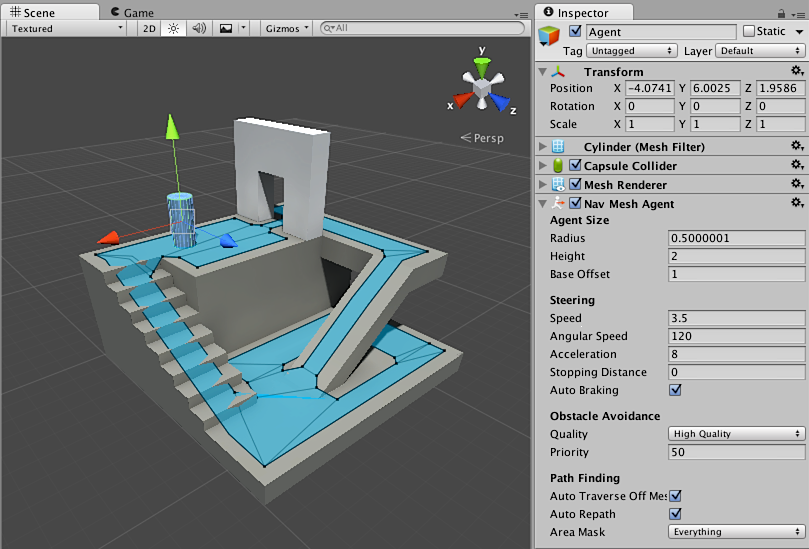
\includegraphics[scale=0.6]{NavMeshImage}
\caption{Exemple d'application du composant \textit{NavMesh} dans Unity. L'agent se déplace à l'intérieur de la zone bleue.}
\end{figure}

\paragraph{}
 Le composant \textit{NavMesh} est un composant d'Unity permettant de déplacer des agents sur des zones (appelé \textit{Navigation Mesh}). Ces zones peuvent avoir différentes propriétés (comme le coût de déplacement) et un algorithme de recherche de plus court chemin est utilisé lorsqu'on demande l'ordre à une unité de se déplacer dans le NavMesh.
\paragraph{}
 Grâce à cela, l'unité était capable de parcourir un chemin jusqu'à arriver à sa destination en évitant les différents obstacles avec lesquelles elle pourrait entrer en collisions, ces dernières étant detectées grâce au composant Collider. M. Ferber nous avait demandé d'étudier la possibilité de créer des zones restrictives, sur lesquelles certaine unité ne seraient pas capables d'aller ou se déplaceraient à une vitesse différente. Cette opération fut simple à mettre en place avec le composant NavMesh, car l'unité peut se déplacer uniquement dans les zones qui lui sont autorisées.
\paragraph{}
Mais l'utilisation du NavMesh ne convenait pas au jeu Warbot. En effet, dans le jeu, l'utilisateur est libre du choix du comportement de l'unité mais doit aussi faire avec les alléa du terrain, et doit prendre en compte la possibilité que l'unité soit bloquée. De ce fait, l'utilisation du composant NavMesh n'est pas judicieux. En effet, ce composant permet de calculer le plus court chemin vers une destination. Cependant, si la destination n'est pas atteignable, le composant NavMesh calcule le point le plus proche dans les zones autorisées de l'unité. Or, cette opération était faite de manière automatique, son utilisation a donc été rapidement abandonnée. 
\paragraph{}
Les zones restrictives ont elles aussi étaient annulées, leur conception sans NavMesh nous ayant parue bien trop complexe et chronophage à ce niveau du projet pour un élément non primordial. 
\paragraph{}
A partir de ce moment, nous avons donc simplement modifié la position du composant Transform (composant determinant la position, rotation et l'échelle de chaque objet dans la scène), du GameObject Unit en fonction du vecteur de mouvement voulu afin de déplacer l'unité.
\paragraph{}
Une fois ces premiers mouvements rendus possibles, on a enfin pu créer notre premier comportement qui consistait à dire à l'unité de bouger si elle n'était pas bloquée.
\begin{lstlisting}[language={[Sharp]C},label={lst:unitScript}, caption=  Extrait du code du script Brain.cs première version.]
    void Update()
    {
        PerceptStructure[] listePercepts = GetComponent<UnitManager>().GetComponent<PerceptManager>()._percepts;
        if (!listePercepts[0]._percept._value) //Percept bloquée? faux
            _actions[0].Do(); // Move
    }

\end{lstlisting}
\paragraph{}
Mais on peut constater que cela nous obligé à écrire l'architecture de subsomption correspondant au comportement en brut, ce qui nuisait à notre besoin de généricité. On s'est donc attardé sur la conception des instructions de l'unité. 
\paragraph{}
Celles-ci furent constituées d'une suite de conditions (percepts) et d'une action terminant le tour de l'unité. La valeur d'un percept était donc calculée à partir d'une fonction booléenne vérifiant les conditions à remplir. Par exemple, le percept de ressource, devant vérifier si une ressource était à proximité. Nous avons commencé par créer la gestion de l'action de la manière suivante : pour créer une action, il fallait hériter de la classe Action et surcharger sa méthode do() en créant l'action voulue.
\paragraph{}Avant de passer à un exemple concret de la gestion d'une instruction, nous allons expliquer comment fonctionnait le champ de vision d'une unité et le calcul des objets "vus" par celle-ci.
Le GameObject Unit a un composant Collider sphérique, une sphère tout autour de lui. Ce Collider détecte tout GameObject à l'intérieur de celle-ci. Dans cette sphère, on décide d'un angle fixe qui sera l'angle de champs de vision de l'unité.
\begin{lstlisting}[language={[Sharp]C},label={lst:unitScript}, caption=  Extrait du code du script Sight.cs première version.]
    void OnTriggerStay(Collider other)
    {
      

        float h = GetComponent<UnitManager>()._stats._heading * Mathf.Deg2Rad;
        Vector3 A = new Vector3(Mathf.Cos(h), 0, Mathf.Sin(h)).normalized * _distance;
        Vector3 B = (other.transform.position - transform.position).normalized * _distance;

        float angle = Vector3.Angle(A, B);
        if (angle <= _angle && !_listOfCollision.Contains(other.gameObject))
        {
            
            _listOfCollision.Add(other.gameObject);
        }
        else if (angle > _angle && _listOfCollision.Contains(other.gameObject))
        {
            _listOfCollision.Remove(other.gameObject);
        }
    }
\end{lstlisting}
Pour la mise à jour de la liste des objets vus par l'unité, on procède comme suit :
\begin{itemize}
\item On récupère la liste des objets présents dans la sphère.
\item Pour tous les objets présents dans la sphère, si celui-ci a sa position dans l'angle de champ de vision de l'unité, on l'ajoute à la liste des objets vus.
\end{itemize}

\begin{lstlisting}[language={[Sharp]C},label={lst:unitScript}, caption=  Classe Instruction du fichier Instruction.cs première version.]
public class Instruction : MonoBehaviour {

    [SerializeField]
    PerceptStructure[] _listePerceptsVoulus;
    [SerializeField]
    Action _action;

    public bool verify()
    {
        PerceptStructure[] listePerceptsUtilisables = GetComponent<UnitManager>().GetComponent<PerceptManager>()._percepts;
        bool verifie = true;
        foreach(PerceptStructure p in _listePerceptsVoulus)
        {
            foreach(PerceptStructure p2 in listePerceptsUtilisables)
            {
                if(p._name.Equals(p2._name))
                {
                    verifie = p2._percept._value;
                }
            }

            if (!verifie)
            {
                break;
            }
        }
        if (verifie)
        {
            _action.Do();
            return true;
        }


        return false;
    }
}
\end{lstlisting}

\paragraph{}Cet exemple montre l'exécution d'une instruction demandant à un agent de récupérer une ressource s'il l'a perçoit, symbolisée par les classes PerceptRessource et ActionPick :
Pour cette instruction on a donc accès à son percept et son action, la vérification des percepts se fait de la manière suivante :
\begin{itemize}
\item On récupère la liste des percepts nécessaires à l'instruction.
\item On récupère la liste des percepts de l'unité.
\item On récupère la valeur de chaque percepts demandés.
\item Si toutes leurs valeurs sont vrai on exécute l'action demandée.
\end{itemize}
\begin{lstlisting}[language={[Sharp]C},label={lst:unitScript}, caption=  Extrait du code du script PerceptRessource.cs première version.]
    override public void update()
    {
        bool res = false;
        foreach (GameObject gO in GetComponent<Sight>()._listOfCollision)
        {
            if (gO && gO.GetComponent<ItemHeldler>())
            {
                GetComponent<Stats>().SetTarget(gO);
                res = true;
                break;
            }
        }
        _value = res;
    }
\end{lstlisting}
La valeur de chaque percept de l'unité est mise à jour à chaque unité de temps, pour PerceptRessource cela se passe comme suit :
\begin{itemize}
\item Pour tous les objets présents dans la liste des objets vus de l'unité.
\item On cherche s'il en existe un qui a un composant "ItemHandler" (ItemHandler est propre aux Prefab de type Ressource cela nous permet de vérifier que l'objet trouvé est bien une ressource).
\item Si c'est le cas on modifie la valeur de la "target" de l'unité (la cible de l'unité pour ce tour de jeu) pour qu'elle soit égale à l'objet trouvé.
\end{itemize}
\begin{lstlisting}[language={[Sharp]C},label={lst:unitScript}, caption=  Extrait du code du script ActionPick.cs première version.]
    public override void Do()
    {
        Objet obj = _target.GetComponent<Objet>();
        Inventory unitInventory = GetComponent<UnitManager>().GetComponent<Inventory>();
        unitInventory.add(obj);
        obj.getPicked();
    }
\end{lstlisting}
L'action de récupération d'un objet par une unité se déroule comme ceci :
\begin{itemize}
\item On récupère le composant Objet de la "target" de l'unité (ce composant est la valeur de l'objet à récupérer).
\item On ajoute cet objet dans le composant inventaire de l'unité.
\item On détruit le GameObjet "target" en utilisant sa méthode getPicked(), qui applique la fonction Destroy(GameObject obj) de Unity (on détruit la représentation physique de l'objet sur la scène).
\end{itemize}
\paragraph{}On vient de voir la récupération d'une ressource par une unité, arrêtons-nous un instant sur le concept et la représentation d'une ressource dans le jeu. Sur Unity, un Prefab est une sauvegarde d'un GameObject avec ses composants et ses propriétés afin que celui-ci puisse être utilisé autant de fois qu'on le souhaite sans avoir à le reconfigurer.

\paragraph{}Du point de vue de sa modélisation, une ressource est représentée par une sphère contenant une autre plus petite en son centre. Elle détient également un système à particules permettant de générer ces dernières, tournant autour du centre de la sphère la rendant plus dynamique. 
\begin{figure}[!h]
\centering
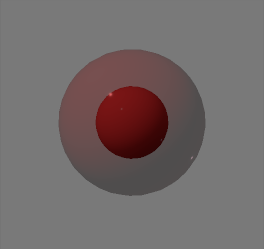
\includegraphics[scale=0.5]{Ressource}
\caption{Une ressource sans son animation.}
\end{figure}
\paragraph{} Pour sa représentation informatique, une ressource est un Prefab détenant un script ItemHandler, uniquement composé d'un attribut de type Objet.
\paragraph{}Le script Objet a donc plusieurs attributs ce qui permet la création d'objet de façon générique utilisable dans le gameplay:
\begin{itemize}
\item Son nom : string \_name.
\item Sa valeur : int \_value.
\item Sa taille : int \_size.
\item Son coût : int \_cost.
\item Sa représentation physique : GameObject \_gameObject.
\item Son script, contenant une unique fonction use(GameObject unit), qui permet de définir la manière dont celui-ci est utilisé par une unité : ItemScript \_itemScript.
\end{itemize}

\paragraph{}
Notre objectif était de simplifier l'ajout de percepts et d'actions à une unité. La définition d'une classe par action et par percept nous semblait donc assez coûteuse nous avons donc étudié l'une des spécificités du C\#.
\paragraph{}
Les types "delegate" propre au C\# ont une déclaration semblable à une signature de méthode.
Elle a une valeur de retour et un nombre quelconque de paramètres de type quelconque.
Nous les avons donc utilisées afin d'encapsuler les méthodes correspondant aux actions et aux percepts et ce afin d'éviter la création de multiples classes.

\begin{lstlisting}[language={[Sharp]C},label={lst:PerceptScript}, caption=  Extrait du code du script Percept.cs]
public abstract class Percept : MonoBehaviour
{
    public delegate bool Listener();
    public Dictionary<string, Listener> _percepts = new Dictionary<string, Listener>();
    [...]
}
\end{lstlisting}

A la suite de ce changement, la classe Percept s'est dotée d'un dictionnaire composée d'une string comme clef et d'un \textit{Listener} comme valeur. Le \textit{Listener} est un delegate représentant la fonction de calcul de valeur du percept. Le même mécanisme est mis en place pour les actions et est toujours d'actualité aujourd'hui.
\paragraph{}L’intérêt d'avoir mis en place un dictionnaire comportant des strings en clefs permet notamment d'obtenir la liste des actions possible de l'unité.

\begin{lstlisting}[language={[Sharp]C},label={lst:unitScript}, caption=  Extrait du code du script PerceptUnit.cs]
 _percepts["PERCEPT_FOOD"] = delegate ()
        {
            GetComponent<Stats>().SetTarget(null);
            foreach (GameObject gO in GetComponent<Sight>()._listOfCollision)
            {
                if (gO && gO.tag == "Item")
                {
                    GetComponent<Stats>().SetTarget(gO);
                    return true;
                }
            }
            return false;
        };
\end{lstlisting}
\begin{lstlisting}[language={[Sharp]C},label={lst:unitScript}, caption=  Extrait du code du script ActionUnit.cs]
_actions["ACTION_PICK"] = delegate () {
            GameObject target = GetComponent<Stats>().GetTarget();
            if (target != null)
                  Objet obj = target.GetComponent<ItemHeldler>()._heldObjet;
                Inventory unitInventory = GetComponent<Inventory>();
                if (!unitInventory.isFull())
                {
                    unitInventory.add(obj);
                    Destroy(target);
                }
            }
        };       {
   
\end{lstlisting}
\subparagraph{Hiérarchisation des actions et des percepts.}
Pour permettre d'éviter la surcharge des classes \textit{Actions} et \textit{Percepts} à destination de plusieurs type d'unités mais comportant plusieurs éléments en commun, nous avons mis en place une hiérarchisation de ces classes. 

\begin{lstlisting}[language={[Sharp]C},label={lst:ActionScript}, caption=  Code du script Action.cs]
public abstract class Action : MonoBehaviour
{
    /*
     * Cette classe abstraite permet de créer de nouvelle action.
     * Pour cela, créer une classe qui dérive de celle-ci.
     */
    public delegate void Act();
    public Dictionary<string, Act> _actions = new Dictionary<string, Act>();
    public abstract void InitAction(); // 
}
\end{lstlisting}

\begin{lstlisting}[language={[Sharp]C},label={lst:ActionCommonScript}, caption=  Code du script ActionCommon.cs dérivant de la classe Action.cs]
public class ActionCommon : Action
{

    void Start(){      
    InitAction();
    }

    public override void InitAction()
    {
        _actions["ACTION_IDLE"] = delegate () { [...] };
        _actions["ACTION_GIVE_RESSOURCE"] = delegate () { [...] };
        _actions["ACTION_HEAL"] = delegate ()  { [...] };
    }
}
\end{lstlisting}

\begin{lstlisting}[language={[Sharp]C},label={lst:ActionUnitScript}, caption=  Code du script ActionUnit.cs dérivant de la classe ActionCommon.cs]
public class ActionUnit : ActionCommon
{
    void Start() {
        InitAction();
    }

    public override void InitAction() {
        base.InitAction(); // IMPORTANT : Permet de récupérer les percepts de la classe mère
        _actions["ACTION_MOVE"] = delegate () { [...] };
        _actions["ACTION_RANDOM_MOVE"] = delegate () { [...] };
        _actions["ACTION_TURN_AROUND_MOVE"] = delegate () { [...] };
        _actions["ACTION_PICK"] = delegate () { [...] };
        _actions["ACTION_BACK_TO_BASE"] = delegate () { [...] };
    }
}
\end{lstlisting}

\paragraph{}
Les listings \ref{lst:ActionScript}, \ref{lst:ActionCommonScript} et \ref{lst:ActionUnitScript} font references à des listes d'actions dans differentes scripts. Lorsqu'on attache le script \textit{ActionUnit} à une unité, les actions possibles pour cette derniere sont toutes les actions qui sont dans la hierachie.
\paragraph{}
Ainsi, les actions \textit{"ACTION\_IDLE"}, \textit{"ACTION\_GIVE\_RESSOURCE"} et \textit{"ACTION\_HEAL"} sont disponibles ayant pour script \textit{ActionUnit} et pour toutes les classes dérivant de celle-ci.

\paragraph{}
Ci-dessous, voici la première représentation du cerveau de l'unité. Le "Brain" a pour but de gérer le comportement de l'unité, c'est-à-dire de vérifier les instructions de celle-ci et de lui donner l'ordre de faire l'action correspondante ce tour. On peut donc voir le mécanisme présenté plus haut, la confirmation de la présence d'une action dans l'instruction ainsi que la vérification des percepts nécessaires à son exécution.

\begin{lstlisting}[language={[Sharp]C},label={lst:firstBrainScript}, caption=  Première version de la classe Brain.cs]
public class Brain : MonoBehaviour
{
    public ActionStructure[] _actions;
    public InstructionScriptable[] _instructions;

    void Update()
    {
        foreach(InstructionScriptable instr in _instructions)
        {
            Action actionPossible = this.actionPossible(instr._stringAction);
            if (actionPossible != null && instr.verify(GetComponent<UnitManager>().GetComponent<PerceptManager>()._percepts))
            {
                actionPossible.Do();
                break;
            }
        }
    }

    public Action actionPossible(string stringAct)
    {
        Action presence = null;
        foreach (ActionStructure actStruc in _actions)
        {
            if (actStruc._name.Equals(stringAct))
            {
                presence = actStruc._action;
            }
        }
        return presence;
    }

}
\end{lstlisting}

\paragraph{}Afin de mener à bien le développement du comportement des unités, on a aussi dû créer une carte plus légère et plus petite que celle de l'ancienne génération nous permettant de faciliter nos tests.


\begin{figure}[h!]
        	\centering
	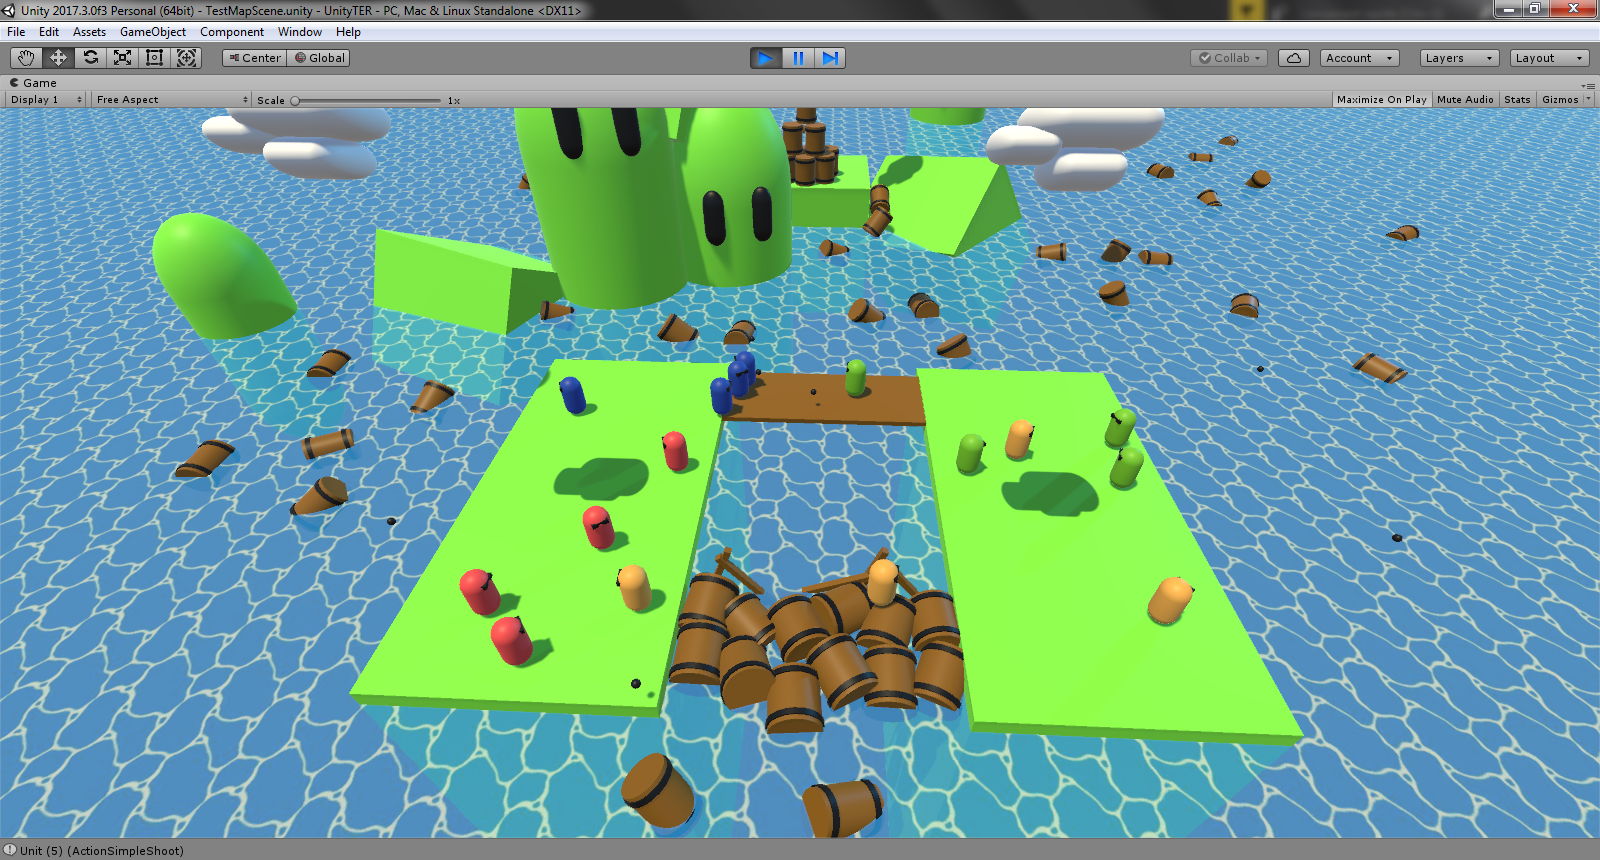
\includegraphics[scale=0.35]{FirstMapImage}
	\caption{Aperçu de la première carte de test.}
\end{figure}

\paragraph{}
Sur cette scène a été introduit le déplacement de la camera principale (MainCamera) calculé en fonction de la position moyenne des unités. Cela permet de donner un effet dynamique à la scène. Ce mécanisme est présent dans le scipt "FollowCamera.cs" attaché à la caméra principale et est toujours d'actualité pour chacune de nos MainCamera de scène de jeu.
\begin{lstlisting}[language={[Sharp]C},label={lst:FollowCamera}, caption=  Extrait du code du script  FollowCamera.cs]
void FixedUpdate ()
    {
        Vector3 res = Vector3.zero;
        GameObject[] units = GameObject.FindGameObjectsWithTag("Unit");

        foreach (GameObject go in units)
        {
            res += go.transform.position;
        }
        res *= 1f / (units.Length + 1);
        currentTarget += (res - currentTarget) * Time.deltaTime * _speed;
        transform.LookAt(currentTarget);
    }
\end{lstlisting}

\paragraph{}
Cette phase de démarrage a duré environ un mois, durant lequel nous avons pu rendre compte chaque semaine à notre encadrant. Durant celle-ci, on a donc agrémenté notre moteur de jeu en suivant les directives de M. Ferber, en nous basant sur notre expérience d'utilisation de Unity pour valider les différents ajouts demandés.

\subsection{Intégration dans le projet.}
Lorsque le moteur nous a paru complet, nous l'avons intégré au projet. Cette phase a été source de problèmes du fait que l'ancien projet était encore présent et que de nombreux conflits persistés.

\subsubsection{Le lien avec l’interpréteur} 
Le plus grand défi de l’intégration était de rendre possible la liaison avec l’interpréteur en place, créé par l'équipe Interpréteur du projet. Nous avons donc travaillé en étroite collaboration avec cette équipe afin de comprendre le fonctionnement de l’interpréteur pour que nous puissions faire les modifications nécessaires.
\paragraph{}Suite à nos échanges, il a été convenu de modifier la classe Instruction qui servira de pont entre l’interpréteur et le moteur.

\begin{lstlisting}[language={[Sharp]C},label={lst:InstructionScript}, caption=  Extrait du code du script Instruction.cs]
public class Instruction {
    public string[] _listeStringPerceptsVoulus;
    public MessageStruct[] _stringActionsNonTerminales;
    public string _stringAction;
    
[...]
   public Instruction(string[] ins, MessageStruct[] actionsNonTerminales, string act)
    {
        _stringAction = act;
        _listeStringPerceptsVoulus = ins;
        _stringActionsNonTerminales = actionsNonTerminales;

    }
[...]
}
\end{lstlisting}
\paragraph{}Cette classe est composée de l'attribut \textit{\_listeStringPerceptsVoulus} correspondant à la liste des labels des percepts de l'instruction, de l'attribut \textit{\_stringActionsNonTerminales} comportant la liste des labels des actions non terminales et d'une string \textit{\_stringAction} qui est le label de l'action à faire. Les actions non terminales ne sont, à ce stade, pas encore implémentées, nous décidons tout de même de les laisser pour les implémenter ultérieurement.
\paragraph{}Lors de la lecture d'un comportement créé par l'éditeur de comportement intégré dans le jeu, l’interpréteur nous renvoie une instance de cette classe Instruction.

\begin{lstlisting}[label={lst:InstructionExample}, caption=  Exemple d'une instruction d'un comportement que peut renvoyer l’interpréteur.]
Instruction (
	Percepts = [PERCEPT_ENEMY, PERCEPT_LIFE_MAX],
	ActionNT = [],
	Action = ACTION_FIRE )
\end{lstlisting}

\paragraph{}L'exemple montrer au listing \ref{lst:InstructionExample} correspond au comportement d'une unité et lui demandera de tirer si l'unité peut percevoir un ennemi, et que sa vie est au maximum. Les actions non-terminales n'étant pas prises en charge à ce moment du développement, la liste est vide. Un comportement n'est donc rien d'autres qu'une liste d'instructions.
\paragraph{}Pour garder l'idée d'une structure de subsomption, la liste des instructions est ordonnée de telle sorte que la première instruction dans cette liste est la première à être examinée et son action est exécutée si ces percepts sont activés.
\subsubsection{Lien avec l'éditeur de comportement.}
Pour permettre au joueur de faire un comportement avec des elements autorisées pour l'unité en question, il nous a fallu transmettre à l'équipe s'occupant de l'editeur graphique les actions et percepts autorisés pour chaque type d'unités.
\paragraph{Les clefs des dictionnaires.} Ainsi chaque unité doit contenir une classe dérivant d'\textit{Action} et de \textit{Percept}.
Ainsi dans l'objet \textit{GameManager}, on renseigne les unités dans la section "List Unit Game Object". Cette section permet de capturer les différentes actions et percepts des différents unités et de les consigner dans un fichier.
\begin{figure}[!h]
\centering
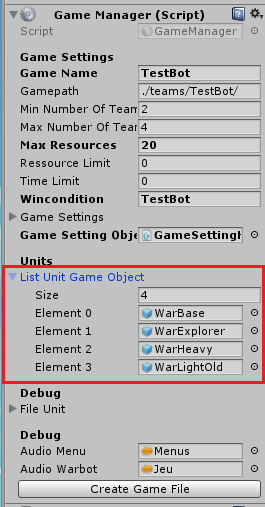
\includegraphics{GameManagerImage}
\caption{Visualisation dans l'\textit{Inspector} d'Unity des unités présentes dans le GameManager.cs}
\end{figure}



\paragraph{}
Ce fichier est repris par l'éditeur de comportement pour créer les pièces de puzzles en fonction des unités.







\subsection{Améliorations des fonctionnalités.}


\subsubsection{Ajout de fonctionnalités des instructions.}
\paragraph{}Un des enjeux du moteur était de pouvoir rendre les instructions plus intéressantes pour le joueur. Il a donc fallu améliorer les instructions qui étaient composées d'une simple liste de percepts, d'actions non terminales et d'une action en rajoutant des fonctionnalités.\newline
\begin{lstlisting}[label={lst:BehaviorExample}, caption=  Exemple d'un comportement que peut renvoyer l’interpréteur.]
Behavior [LIGHT] = {
1. Instruction (  Percepts = [PERCEPT_ENEMY, PERCEPT_LIFE_MAX],
		ActionNT = [],
		Action = ACTION_FIRE ),
2. Instruction (  Percepts = [PERCEPT_ENEMY, NOT_PERCEPT_LIFE_MAX],
		ActionNT = [MESSAGE_HELP(@ HEAVY)],
		Action = none),
3. Instruction (  Percepts = [ NOT_PERCEPT_LIFE_MAX],
		ActionNT = [],
		Action = ACTION_HEAL ),
4. Instruction (  Percepts = [],
		ActionNT = [],
		Action = ACTION_MOVE ) }
\end{lstlisting}


\paragraph{}Le comportement défini en listing \ref{lst:BehaviorExample} comporte plusieurs instructions  résumant les possibilités du moteur.

\paragraph{1. Négation.}
La plus grande amélioration que l'équipe de Game Design nous avait demandé d'apporter au moteur sur le plan des instructions était de mettre en place la négation des percepts.
\subparagraph{} Pour rappel, un percept est une fonction anonyme qui renvoie un booléen. La composition de plusieurs percepts donne l'illusion d'un tableau de bord, permettant à l'unité de se faire une idée de son environnement. Cependant, les instructions fonctionnent actuellement en utilisant une liste conjonctive de percepts. En d'autres termes, tout les percepts d'une instruction doivent être activés pour pouvoir exécuter l'action de l'instruction.
\subparagraph{}Il nous fallait donc trouver un moyen pour rendre possible la négation des percepts. Ainsi, en travaillant de concert avec l'équipe Interpréteur, nous avons convenu d'un préfixe \textit{NOT\_} que l'on concatène au label des percepts, comme vu aux instructions 2. et 3. du listing \ref{lst:BehaviorExample}.
\begin{lstlisting}[label={lst:BehaviorExampleNeg}, caption = Un percept et son inverse.]
PERCEPT_LIFE_MAX; //Activé lorsque "TRUE"
NOT_PERCEPT_LIFE_MAX; //Activé lorsque "FALSE"
\end{lstlisting}

\subparagraph{}En utilisant cette manière, on permet à l'éditeur de comportement de transcrire le choix du joueur (négation ou pas) via un fichier XML que l’interpréteur peut traduire en \textit{Instruction} pour notre moteur.

\begin{lstlisting}[language={[Sharp]C},label={lst:VerifyBrainScript}, caption=  Extrait du code du script Brain.cs]
public class Brain : MonoBehaviour
{
[...]
bool Verify(Instruction instruction)
    {
        bool flag = true;
        foreach (string percept in instruction._listeStringPerceptsVoulus)
        {
            if (!(_componentPercepts._percepts.ContainsKey(percept.Replace("NOT_", "")) && 
                (percept.Contains("NOT_") ^ _componentPercepts._percepts[percept.Replace("NOT_", "")]())))  { flag = false; }
        }
        return flag;
    }
[...]
}
\end{lstlisting}

\subparagraph{}Pour rendre le moteur compatible avec la négation des percepts, on a du modifier la fonction \textit{Verify} (listing \ref{lst:VerifyBrainScript}) du script Brain.cs. Cette fonction vérifie si une instruction donné en paramètre est activé. On regarde ainsi si tout les percept sont activés. \newline
Ainsi, une instruction est activé si :
\begin{itemize}
\item Il existe le percept dans la liste des percepts de l'unité. (En enlevant le préfixe \textit{NOT\_}).
\item Le percept ne contient pas le préfixe \textit{NOT\_} et le percept renvoie "TRUE".
\item Le percept contient le préfixe \textit{NOT\_} et le percept renvoie "FALSE".
\end{itemize}
\paragraph{2. Actions non-terminales.}
Pour permettre une plus grande liberté dans la conception des comportements des unités, il a était rapidement nécessaire de rajouter des actions dites \textit{non-terminales}. Ces actions sont effectuées au même titre que les actions terminales à la différence près que celle-ci n’empêche pas d’exécuter une autre instruction située hiérarchiquement plus bas dans l'architecture de subsomption si l'instruction ne comporte pas d'action terminant le tour de l'unité.

\begin{lstlisting}[language={[Sharp]C},label={lst:ActionNonTerminalScript}, caption=Code du script ActionNonTerminal.cs]
using System.Collections;
using System.Collections.Generic;
using UnityEngine;

public abstract class ActionNonTerminal : MonoBehaviour
{
    public delegate void ActNonTerm();
    public Dictionary<string, ActNonTerm> _actionsNT = new Dictionary<string, ActNonTerm>();
    public abstract void InitActionNonTerminal();
    public string _messageDestinataire;
    public Message _tmpMessage;
}

\end{lstlisting}
\paragraph{}
Comme pour les actions terminales et les percepts, les actions non-terminales sont constituées d'un dictionnaire composé de chaîne de caractères comme clef et un delegate \textit{ActNonTerm} correspondant à la méthode anonyme de l'action non-terminal.

\begin{lstlisting}[language={[Sharp]C},label={lst:ActionNonTerminalExempleScript}, caption=Exemple d'une action non-terminale]
        _actionsNT["ACTN_HEADING_RANDOM"] = delegate ()
        {
            GetComponent<Stats>().SetHeading(Random.Range(0f,360f));
        };
\end{lstlisting}

\paragraph{}
Dans le listing \ref{lst:ActionNonTerminalExempleScript}, on peut voir l'exemple d'une action non-terminale. Fonctionnant comme une action classique, l'action non-terminale \textit{"ACTN\_HEADING\_RANDOM"} permet à une unité de faire une rotation aléatoire.
\subparagraph{Messages.}
Les messages sont des actions non-terminales particulieres. En effet, ces actions possedent un argument correspondant au destinataire du message.

\begin{figure}[!h]
       \centering
	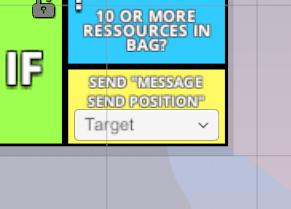
\includegraphics[scale=0.55]{PuzzleMessageImage}
	\caption{Représentation des messages dans l'éditeur.}
\end{figure}

\subparagraph{} 
Pour representer les messages dans le moteur, nous avons créé une liste de la struct \textit{MessageStruct}.

 \begin{lstlisting}[language={[Sharp]C},label={lst:MessageStructScript}, caption= Code du script MessageStruct.cs]
public class MessageStruct {
    public string _intitule;
    public string _destinataire;
    public MessageStruct(string intitule, string destinataire)
    {
        _intitule = intitule;
        _destinataire = destinataire;
    }
}
\end{lstlisting}

\paragraph{}
Cette structure est composé simplement de deux attributs string \textit{\_intitule} correspondant au titre ou au contenu du message et string \textit{\_destinataire} qui correspond à/aux unité(s) dont le message est destiné. Les destinataires peuvent etre :
\begin{itemize}
\item La cible courante.
\item A tous.
\item A un type d'unité en particulier.
\end{itemize}

\paragraph{3. Mouvements tactiques.}
Comme définie dans le listing \ref{lst:BehaviorExample}, l'instruction 2. permet de faire une action non-terminale même sans d'action terminale.
Ainsi on a la possibilité de réaliser des mouvements plus tactiques sans terminer le tour.
\paragraph{}Lorsque les percepts de l'instruction 2 sont activés, cela déclenche l'action non terminale en ligne 6 qui envoie un message d'aide aux unités de type \textit{Heavy}. Mais comme il n'y a pas d'action terminant le tour, on continue à regarder les autres instructions tant qu'il n'y a pas d'action terminale à effectuer.

\paragraph{4. Instructions par défaut.}
Lorsqu'une instruction ne comporte pas de percepts, cette instruction est, par définition toujours valide. Cela permet, entre autre, de créer des cas par défaut que l'on peut mettre à la fin d'un comportement. L'action de cette instruction est alors toujours exécutée si aucune autre action ne peut l'être.

\paragraph{5. Cas exceptionnels.}
Dans un comportement, il peut arriver que les conditions de toutes les instructions soient fausse, empêchant ainsi l'exécution d'une action. Dans ce cas précis, c'est le moteur qui choisi l'action à effectuer. Actuellement, l'unité exécute l'action \textit{ACTION\_IDLE}.

\subsubsection{Gestion des messages.}
L'une des fonctionnalités importantes liées aux systèmes multi-agents est le fait que les agents puissent s'envoyer des signaux (représenter dans notre projet par des messages) entre eux afin de réaliser des tâches de plus grandes importance où la cohérence de groupe est nécessaire. Nous avons donc mis en place un système de messagerie entre robot que l'utilisateur peut utiliser pour créer des comportement plus évolués.

\paragraph{Messagerie individualisée.} 
Afin de permettre une gestion des messages, nous nous sommes tout naturellement tourné vers une messagerie individualisée.
 \begin{lstlisting}[language={[Sharp]C},label={lst:MessageManagerScript}, caption= Code du script MessageManager.cs]
public abstract class MessageManager : MonoBehaviour
{
	[...]
    public List<Message> _waitingMessages = new List<Message>();
    public List<Message> _currentMessages = new List<Message>();
	[...]
    public void UpdateMessage()
    {
        _currentMessages = _waitingMessages;
        _waitingMessages = new List<Message>();
    }
	[...]
}
\end{lstlisting}
\paragraph{}
Lorsqu'un message est envoyé à une unité, ce message est recuperé dans le \textit{MessageManager} de l'unité et est réceptionné dans la liste de messages \textit{\_waitingMessages}. Cette liste reçoit tous les messages du tour en cours de l'unité. Ce système a été mis en place pour éviter que certaines unités reçoivent des messages avant d'autres.
\paragraph{}
Dans le script \textit{Brain.cs} (listing \ref{lst:BrainScript}), la méthode \textit{UnitTurn} s'occupe de la gestion du tour de l'unité. La première phase du tour fait appelle à \textit{UpdateMessage()} du composant \textit{MessageManager}. Cette méthode met à jour la liste des messages en basculant les messages de la liste d'attentes (\textit{\_waitingMessages}) dans la liste de messages courants (\textit{\_currentMessages}).
\subsubsection{Gestion des contrats.}
Les unités ont une "target", qui est leur cible pour le tour actuel. Celle-ci peut être un ennemi sur lequel l'unité doit tirer, une ressource qu'elle doit récupérer...
\newline Maiis un des ajout important dans ce projet a été la notion d'objectif, de cible à long terme. Celle-ci est représentée par un contrat. Un contrat est un engagement pris par une unité envers une autre. Par exemple si une unité repère un ennemi sur la carte et qu'elle souhaite demander du renfort, elle peut envoyer un message proposant un contrat à certaines unités et celles-ci peuvent l'accepter. Dans ce cas, l'ennemi repéré devient la cible au long terme de l'unité, cela signifie que l'unité détient l'identité de l'ennemi qui reste en mémoire jusqu'à ce que celui-ci meurt ou que l'unité accepte un nouveau contrat. Ce mécanisme est mis en place de manière générique et un type de contrat spécifique "EliminationContract" est actuellement en place, celui-ci reprend le principe de l'exemple ci-dessus. Le même type de contrat pourrait donc être utilisé à fin de demender la récupération de ressource ou encore de demander de l'aide à d'autres unités alliées. Les unités ont donc accès au message "AttackUnit", proposant un contrat; au percept "HaveEliminationContract", vérifiant la détention d'un contrat d'élimination et à l'action non terminale "AddEliminationContract" lui permettant d'accepter un contrat.     

\subsubsection{Optimisation du temps de chargement.}
\paragraph{} L'un des gros problèmes que l'on a rencontré est le fait que le temps de chargement lors d'une partie était beaucoup trop élevé. Cela nuisait au bon déroulement de la partie, atteignant parfois deux minutes de temps de chargement lorsque l'on voulait générer 200 unités. Pour résoudre ce problème, nous avons étudié plusieurs pistes.
\subparagraph{1. La gestion des actions des unités.}La première piste de recherche que l'on a étudié est d'essayer d'optimiser la gestion des actions des unités. Lorsque l'on a conçu les unités, elles faisaient leurs actions dans une fonction propre à Unity ("Update") qui est appelée à chaque calcul d'image. Ainsi, pour chaque unité présente sur la scène, Unity calcule l'action qu'elle doit faire. Cependant, certaines actions nécessitent plus de temps en fonction de leur complexité, ce qui pouvait engendrer que des unités avaient des tours de retard par rapport à d'autres unités. \newline
Pour palier à ce problème, nous avons donc délégué la gestion des tours des unités à un script  "TurnManagerScript.cs" (Listing \ref{lst:turnManagerScript}).\newline

 \begin{lstlisting}[language={[Sharp]C},label={lst:turnManagerScript}, caption= Code du script TurnManagerScript.cs]
using System.Collections;
using System.Collections.Generic;
using UnityEngine;

public class TurnManagerScript : MonoBehaviour
{
    public float _timeTick;
    public float _ticksPerSeconds;
    
    // Update is called once per frame
	void FixedUpdate ()
    {
        _timeTick += 0.02F * Time.timeScale;
        _ticksPerSeconds = (1.0f / 0.02F) * Time.timeScale;
        if (_timeTick >= 0.04f) // Est-ce que 0.4 secondes ce sont écoulées ?
        {
            _timeTick -= 0.04f;

            foreach (GameObject unit in GameObject.FindGameObjectsWithTag("Unit"))
            {
                if (unit.GetComponent<Brain>()) // Comporte un "Brain"
                {
                    unit.GetComponent<Brain>().UnitTurn(); // Fait l'action de l'unité
                }
            }
        }
	}
}
\end{lstlisting}
Ce script permet de contrôler le fait que chaque unité ne commence pas un nouveau tour si d'autres unités n'ont pas fini ou fait le leurs.
Cependant, cette optimisation n'a pas permis de réduire le temps de chargement d'une partie, restant toujours à prés de deux minutes pour la génération de 200 unités.

\subparagraph{2. \textit{ObjectPool}, les "bassins" d'objets.}Pour essayer de mieux localiser le problème, nous avons effectué des tests sur le temps de chargement en fonction du nombre d'unités. Les résultats sont consignés dans le tableau ci-dessous. On peut donc voir que le nombre d'unité à générer influe directement sur le temps de chargement.\newline
\begin{center}
\begin{tabular}{c|c}
  \hline
  Nombre d'unités à générer & Temps de chargements (moyenne de 3 tests) \\
  \hline
  0 unité & 0.49 secondes \\
  1 unité & 0.70 secondes \\
  5 unités & 3.13 secondes \\
  20 unités & 11.50 secondes \\
  50 unités & 27.84 secondes \\
  100 unités & 50.23 secondes \\
  200 unités & 162.20 secondes \\
  500 unités & 276.71 secondes \\
  \hline
\end{tabular}
\end{center}
Pour empêcher la génération des unités pendant le temps de chargement, nous avons décidé d'utiliser une méthode dite "du bassins d'objets" (ou \textit{ObjectPooling}). Cette méthode consiste à créer un ensemble d'objets dans un objet appelé \textit{Pool}, puis de les rendre inactifs pour que les scripts contenus dans ces objets ne soient pas exécutés.

%% CODE %%
 \begin{lstlisting}[language={[Sharp]C},label={lst:structPoolScript}, caption= Code de la structure \textit{Pool} de ObjectPool.cs]
public struct Pool
{
    public string tag; // Label du Pool
    public int number; // Nombre d'objets
    public GameObject prefab; //Objet de référence
}
\end{lstlisting}

Cette méthode permet de ne pas créer une unité directement, mais de juste prendre un objet Unit dans le bassin correspondant. Les bassins sont représentés par une structure définit au listing \ref{lst:structPoolScript}. Elle comporte un \textit{tag} représentant le nom du bassin, un  \textit{number} correspondant au nombre d'unités à créer dans ce bassin, et enfin un \textit{prefab} qui est l'objet qui servira de référence pour la copie des objets. Le script ObjectPoolScript.cs (Listing  \ref{lst:ObjectPoolScript}) permet la gestion de plusieurs \textit{Pools}, et dans notre cas, nous utilisons 3 \textit{Pools}:  \textit{Light},  \textit{Heavy} et  \textit{Explorer}.

\begin{figure}[!h]
\centering
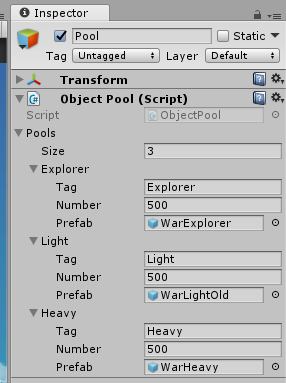
\includegraphics{ObjectPoolingImage}
\caption{Visualisation dans l'\textit{Inspector} d'Unity des \textit{Pools} du script ObjectPool.cs}
\end{figure}

\subparagraph{} Cependant, le temps de chargement est sensiblement le même en utilisant ce principe. Le problème vient donc de la conception même des objets des unités. \newline
Pour trouver d’où viens précisément le problème, on a donc décidé de créer 200 unités et de désactiver certains composants. En utilisant ce procédé, on a pu découvrir et comprendre l'origine du problème.

\subparagraph{3. Simplification des collisions.} La gestion des collisions entre unités et l'environnement se faisait avec un \textit{MeshCollider}. Le \textit{MeshCollider} est un composant de type \textit{Collider} qui permet la gestion des collisions notamment en envoyant des messages aux différents acteurs de la collision. Le \textit{MeshCollider} à la particularité d'épouser plus ou moins la forme du maillage de l'objet que l'on met en argument.
\begin{figure}[!h]
\centering
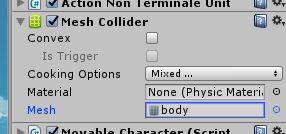
\includegraphics{MeshColliderImage}
\caption{Un composant \textit{MeshCollider}}
\end{figure}
\subparagraph{}Néanmoins, le \textit{MeshCollider} est un composant gourmand en ressource pour calculer les potentiels collisions avec son environnement et, surtout, les maillages que nous utilisons comportent un nombre relativement conséquent de points et de faces. Nous avons résolu ce problème en supprimant les composants \textit{MeshCollider} des unités en les remplaçant par des  \textit{BoxColliders}. Les \textit{BoxColliders} sont des composants de type \textit{Collider}, qui permet la gestion des collisions. Ce composant est définit par un pavé ce qui réduit considérablement les calculs pour connaître les éventuelles collisions avec celui-ci.

\begin{figure}[!h]
\centering
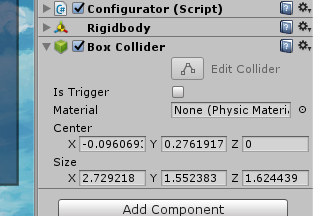
\includegraphics{BoxColliderImage}
\caption{Un composant \textit{BoxCollider}}
\end{figure}

\subparagraph{}Effectivement, le temps de chargement est considérablement réduit, passant de plus de 4 minutes pour 500 unités à une poignée de secondes.



\subsubsection{Amélioration des collisions.}
\paragraph{} Après avoir découvert et réglé le problème de chargement des parties. Nous avons remarqué de nombreux bugs par rapport aux collisions des unités. En effet, certaines unités ne reconnaissaient pas l'environnement et traversaient le décor. Pour résoudre ce problème, nous avons donc définit certaines règles de collisions.
\begin{enumerate}
\item Une unité rentre en collision si un objet est devant lui. 
\item Une unité rentre en collision si l'angle du point de collision par rapport a un autre objet est inférieur à 90°.
\end{enumerate}

 \begin{lstlisting}[language={[Sharp]C},label={lst:MovableCharacterCollisionScript}, caption= Extrait du code de MovableCharacter.cs]
public class MovableCharacter : MonoBehaviour
{
[...]
    void OnCollisionStay(Collision other)
    {
        collisionObject = null;
        if (other.gameObject.tag != "Ground")
        {
            foreach (ContactPoint contact in other.contacts)
            {
                float a = Utility.getAngle(gameObject.transform.position, contact.point);
                float b = GetComponent<Stats>().GetHeading();
                float A = Mathf.Abs(a - b);
                float B = Mathf.Abs( 360+ Mathf.Min(a,b) - Mathf.Max(a, b) ) ;
                if (Mathf.Min(A, B) < 90f)
                {
                    collisionObject = other.transform.gameObject;
                    break;
                }
            }
        }
    }
[...]
}
\end{lstlisting}
\subparagraph{} Dans l'extrait du code ci-dessus, on peut voir que l'objet qui est en collision avec l'objet est mis à jour seulement si l'angle est inférieur à 90°. Pour éviter de rentrer en collision avec le sol, l'objet ne doit pas comporter le \textit{tag} "Ground".



\section{Usage.}
Le sujet de notre projet est de permettre à des programmeurs de pouvoir concevoir un jeu orienté multi-agents en fournissant des outils générique. Dans cette section, nous allons décrire les opérations nécessaires pour réaliser un jeu multi-agents dans le moteur de jeu Unity.
\subsection{Prérequis.}
\paragraph{Le moteur Unity.}Pour permettre la création d'un jeu orienté-agents, nous avons utilisé le moteur de jeu Unity. Comme dit précédemment, le moteur Unity 3D est un logiciel de création de jeu. Il est convenable d'avoir des notions sur ce moteur de jeu. En effet, Unity nécessite appréhender des notions qui lui sont propres.
\paragraph{}De nombreux exemples et tutoriels sont disponible sur internet, notamment sur le site du développeurs. Pour plus d'informations, nous vous conseillons les sites:
\begin{itemize}
\item Le site officiel d'Unity 3D : https://unity3d.com/fr
\item La page de téléchargement d'Unity : https://store.unity.com/
\item La documentation officielle d'Unity : https://docs.unity3d.com/Manual/index.html
\end{itemize}


\subsection{Création d'unité.}
Pour pouvoir créer une unité simplement, nous avons mis en place des scripts pour permettre cela.
Toutes les unités doivent avoir les 8 scripts suivant:
\begin{figure}[!h]
\centering
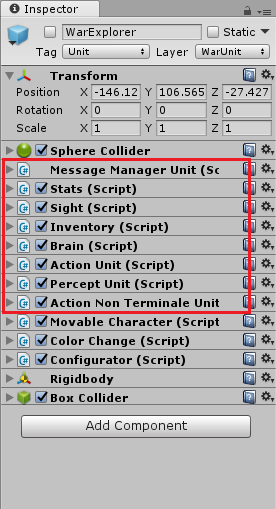
\includegraphics[scale = 0.5]{WarUnitImage}
\caption{Un exemple de la composition d'une unité.}
\end{figure}

\begin{itemize}
\item \textit{Message Manager Unit.} Le gestionnaire des messages.\newline
Ce script permet la gestion des messages de l'unité. Il gère aussi les types de messages que l'unité peut envoyer. 

\item \textit{Stats.} Les statistiques.\newline
Ce script donne accès aux statistiques de l'unité. (Listing \ref{lst:LoadFile}).
\item \textit{Sight.} Le champ de vision.\newline
Permet à l'unité de se représenter son environnement.  
\begin{figure}[!h]
\centering
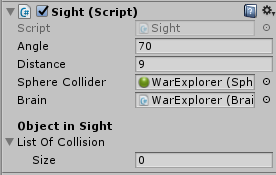
\includegraphics[scale=0.75]{SightScriptImage}
\caption{Composant Sight d'une unité.}
\end{figure}



\item \textit{Inventory.} L'inventaire.\newline
Donne la possibilité à une unité de stocker des objets. L'inventaire est caractérisé par le nombre maximal d'objets qu'il peut contenir.
\begin{figure}[!h]
\centering
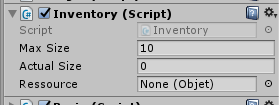
\includegraphics{InventoryImage}
\caption{Composant Inventory d'une unité.}
\end{figure}


\item \textit{Brain.} Le centre de commandement de l'unité. (listing \ref{lst:BrainScript})
\item \textit{Action Unit.} La liste des actions autorisés de l'unité.
\item \textit{Percept Unit.} La liste des percepts accessible de l'unité.
\item \textit{Action Non Terminale Unit.} La liste des actions non-terminales possible de l'unité.
\end{itemize}



\subsection{Création de carte.}
\paragraph{Le nécessaire MetaBot.} Pour simplifier la création d'une scène dans MetaBot, nous avons rassembler les scripts et GameObject important dans un seul est même contenant. \textit{\_MetaBotNecessary}.

\begin{figure}[!h]
\centering
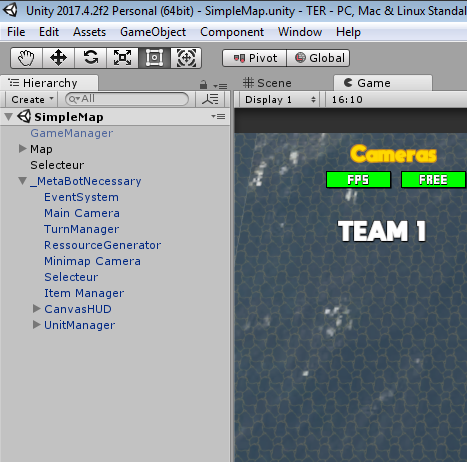
\includegraphics[scale=0.55]{MetaBotNecessaryImage}
\caption{Hierarchie des \textit{GameObjects} de la scène \textit{Simple}}
\end{figure}

\begin{itemize}
\item \textit{MainCamera.} La caméra principale où est affichée les éléments de l'interface graphique lors d'une partie.

\begin{figure}[!h]
\centering
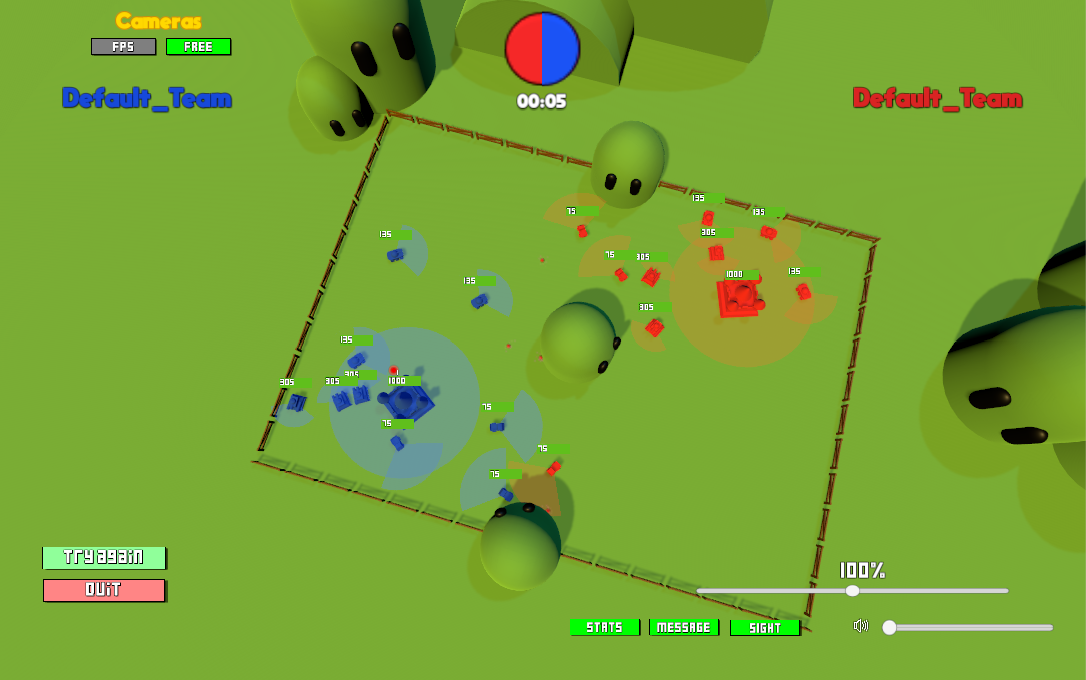
\includegraphics[scale=0.5]{Screenshot001}
\caption{Rendu de la caméra principale lors d'une partie}
\end{figure}

\item \textit{TurnManager.} S'occupe de la gestion des tours des unité.


\item \textit{RessourceGenerator.} Cet objet permets de générer les ressources nécessaires au jeu WarBot.


\begin{figure}[!h]
\centering
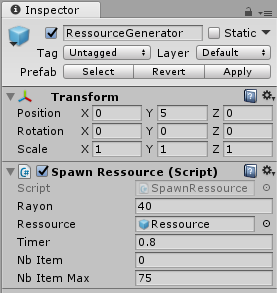
\includegraphics[scale=0.85]{RessourceGeneratorImage}
\caption{Script \textit{SpawnRessource.cs} dans l'éditeur d'Unity}
\end{figure}

\item \textit{MinimapCamera.} Caméra permettant l'affichage de la mini-carte en mode vue subjective.
\item \textit{ItemManager.} Gère le comportement des objets.
\item \textit{CanvasHUD.} Le canvas permettant d'afficher les éléments graphiques sur la caméra. Il contient notamment les scores, les noms des équipes, la gestion du temps, et les boutons de contrôle.
\item \textit{UnitManager.} Gestionnaire d'unité qui comporte les 4 équipes. C'est ici que le positionnement des unités de départ est géré. Ainsi les bases des équipes 

\begin{figure}[!h]
\centering
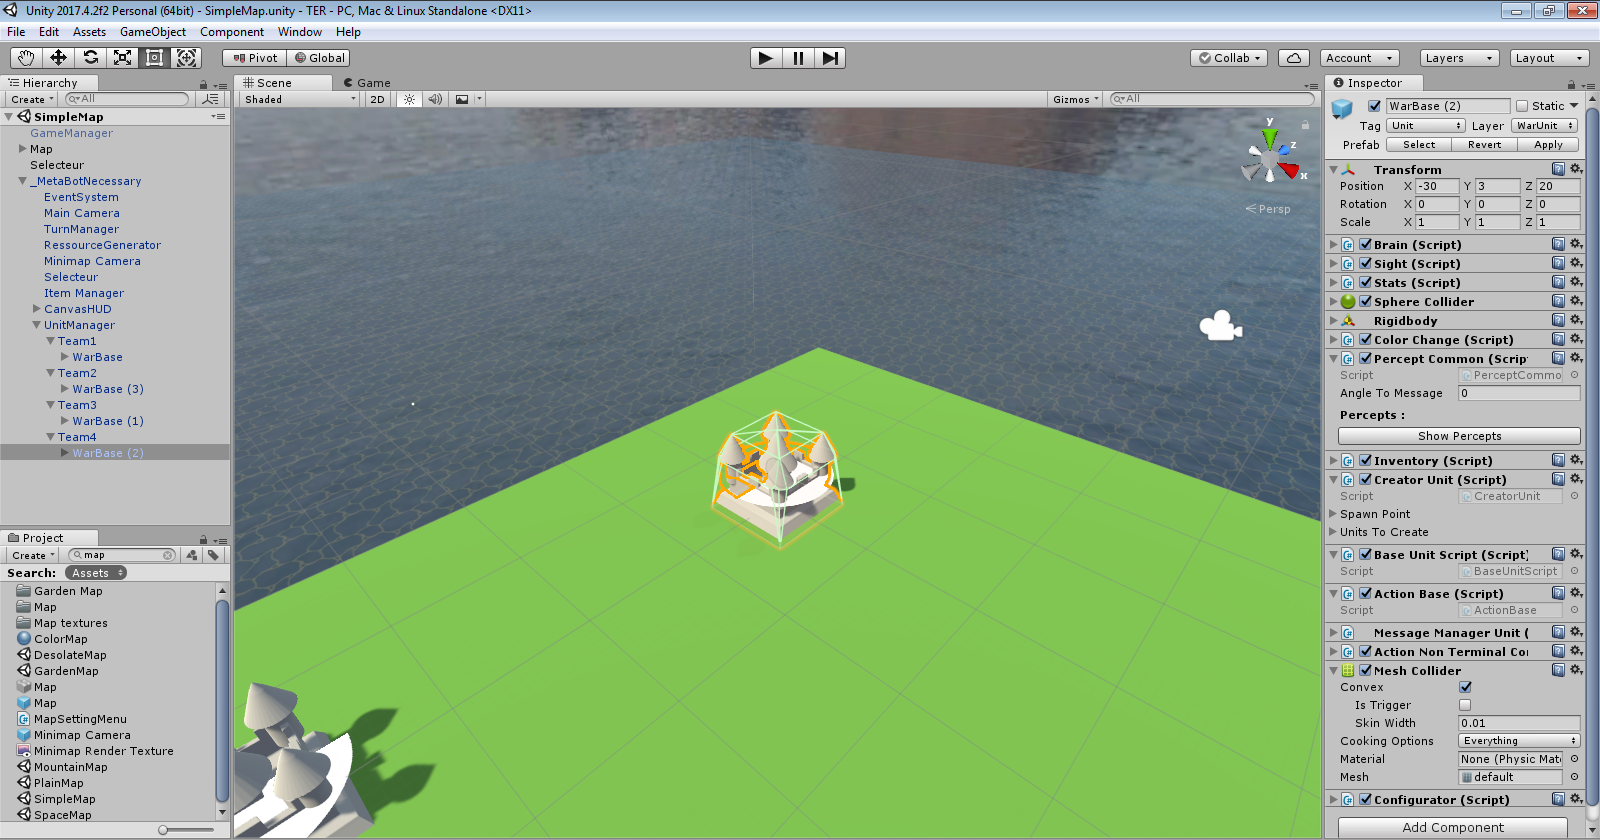
\includegraphics[scale=0.25]{UnitManagerImage}
\caption{Le positionnement d'une base dans la scene.}
\end{figure}

\end{itemize}

\subsection{Gestion des comportements.}
\paragraph{Action, Action non-terminales et Percepts.}
Pour ajouter de nouvelles actions, actions non-terminales et percepts, il faut créer des classes dérivant des classes \textit{Action}, \textit{ActionNonTerminal} et \textit{Percept}.

 \begin{lstlisting}[language={[Sharp]C},label={lst:ActionUnit2Script}, caption= Code de ActionUnit.cs]
public class ActionUnit : ActionCommon {
    void Start() {
        InitAction();
    }
    
    public override void InitAction() {
        base.InitAction(); // IMPORTANT : Permet de recuperer les percepts de la classe mere
        _actions["ACTION_MOVE"] = delegate () { GetComponent<MovableCharacter>().Move(); };
        
        _actions["ACTION_RANDOM_MOVE"] = delegate ()
        {
            GetComponent<Stats>().SetHeading(Random.Range(0f,360f));
            _actions["ACTION_MOVE"]();
        };
   
        _actions["ACTION_TURN_AROUND_MOVE"] = delegate () { [...] };
        _actions["ACTION_PICK"] = delegate () { [...] };
        _actions["ACTION_BACK_TO_BASE"] = delegate () { [...] };
    }
}
\end{lstlisting}


\paragraph{Squelettes.}Ci-dessous, les trois squelettes pour l'ajout d'actions, d'actions non-terminales et de percepts.
 \begin{lstlisting}[language={[Sharp]C},label={lst:ActionNewScript}, caption= Structure du code d'une nouvelle classe d'action.]
public class ActionNew : Action {

    void Start() 
    {
        InitAction();
    }
    
    public override void InitAction() 
    {
        base.InitAction(); // IMPORTANT : Permet de récupérer les actions de la classe mère
        /* Code à définir ici */
    }
}
\end{lstlisting}

 \begin{lstlisting}[language={[Sharp]C},label={lst:PerceptNewScript}, caption= Structure du code d'une nouvelle classe de percepts.]
public class PerceptNew : Percept {

    void Start() 
    {
        InitPercept();
    }
    
    public override void InitPercept() 
    {
        base.InitPercept(); // IMPORTANT : Permet de récupérer les percepts de la classe mère
        /* Code à définir ici */
    }
}
\end{lstlisting}

 \begin{lstlisting}[language={[Sharp]C},label={lst:ActionNonTerminalNewScript}, caption= Structure du code d'une nouvelle classe d'action non-terminale.]
public class ActionNonTerminalNew : ActionNonTerminal {

    void Start() 
    {
       InitActionNonTerminal();
    }
    
    public override void InitActionNonTerminal()
    {
        base.InitActionNonTerminal(); // IMPORTANT : Permet de récupérer les actions non-terminales de la classe mère
        /* Code à définir ici */
    }
}
\end{lstlisting}

\section{Modélisation 3D, sons et animation.}

\subsection{Les unités Warbot.}
Afin de pouvoir tester les fonctionnalités que nous avons mis en place, nous avons créer des unités. On a ainsi du concevoir des modèles 3D pour les unités en utilisant le logiciel libre de droit \textit{Blender}.

\begin{figure}[h]
    \begin{minipage}[c]{.46\linewidth}
        \centering
        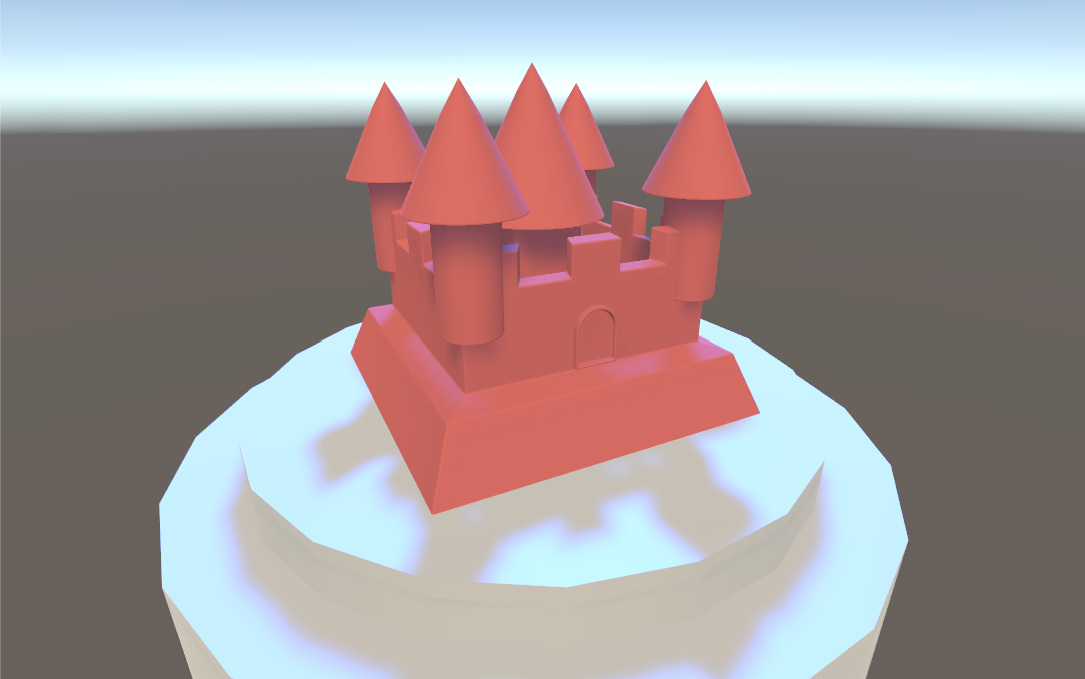
\includegraphics[scale=0.25]{WarBaseImage}
        \caption{L'unité Base de WarBot.}
    \end{minipage}
    \hfill%
    \begin{minipage}[c]{.46\linewidth}
        \centering
        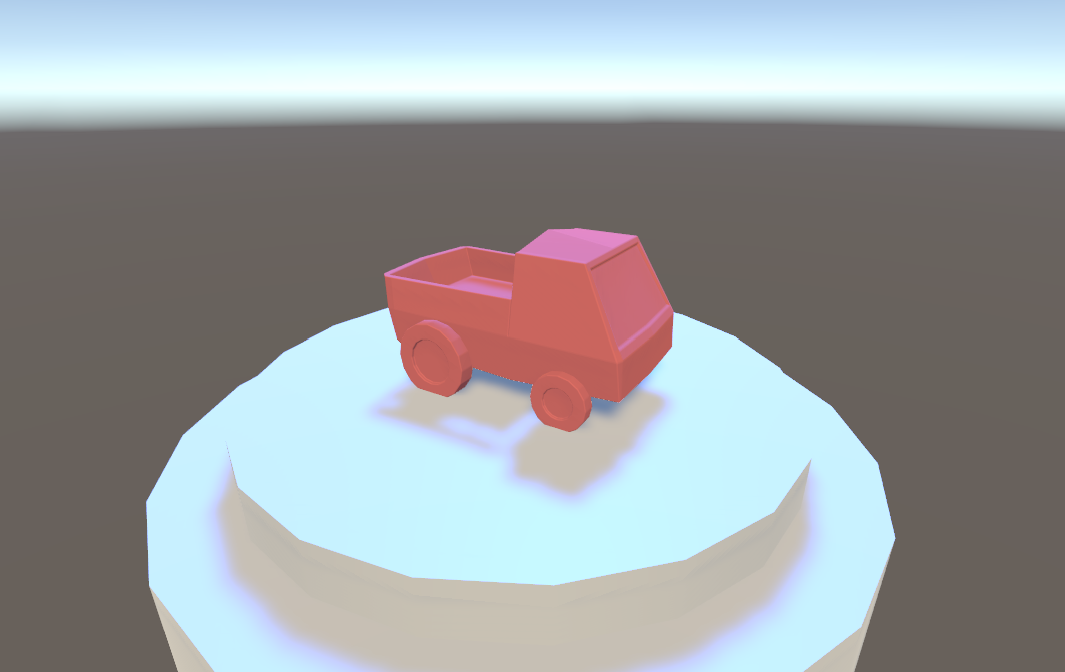
\includegraphics[scale=0.25]{WarExplorerImage}
        \caption{L'unité Explorer de WarBot.}
    \end{minipage}
\end{figure}
\begin{figure}[h]
    \begin{minipage}[c]{.46\linewidth}
        \centering
		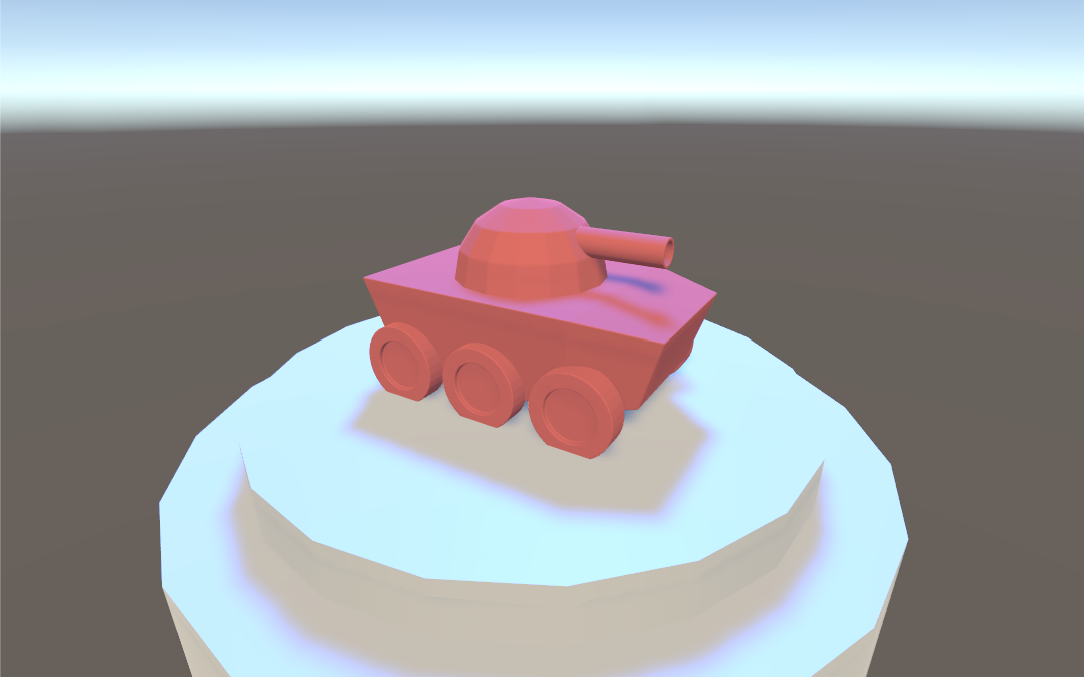
\includegraphics[scale=0.25]{WarLightImage}
	\caption{L'unité Light de WarBot.}
    \end{minipage}
    \hfill%
    \begin{minipage}[c]{.46\linewidth}
        \centering
		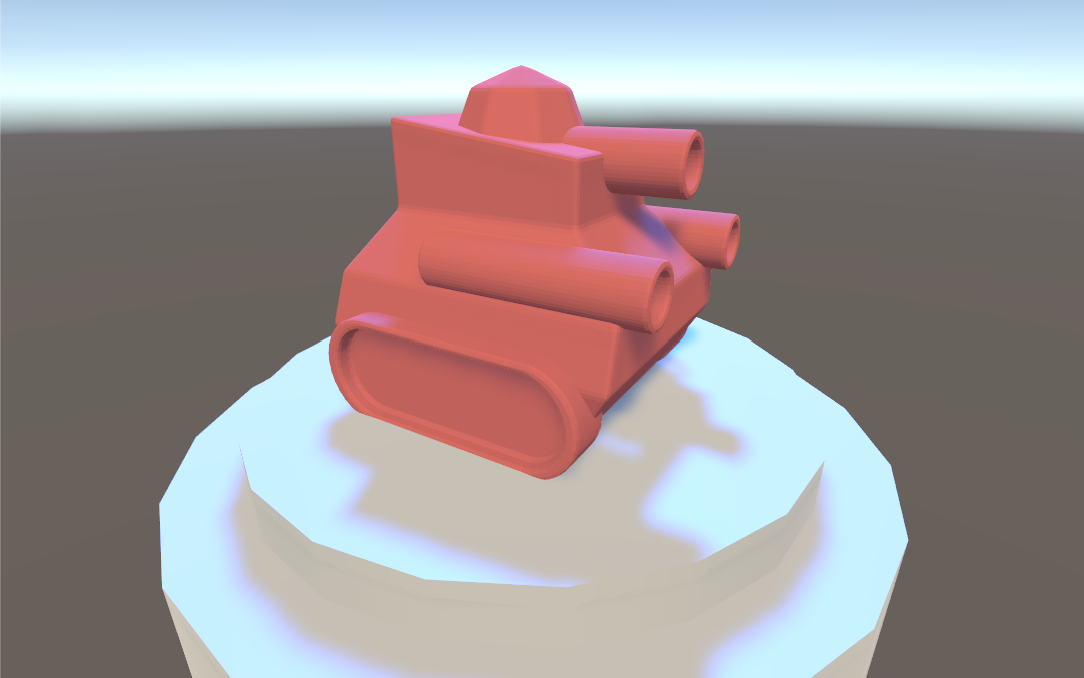
\includegraphics[scale=0.25]{WarHeavyImage}
	\caption{L'unité Heavy de WarBot.}
    \end{minipage}
\end{figure}

\newpage
\subsection{Les différentes cartes.}
Pour tester les unités, nous avons conçu 5 différentes cartes.
\begin{itemize}
\item \textit{Simple}: Carte basique ne comportant pas d'obstacle. C'est une île rectangulaire entourée d'eau.
\item \textit{Mountain}: Une île plus élaboré ayant des bords plus irréguliers comportant une chaîne de montagne au sud-est de la carte.
\item \textit{Desolate}: Un désert avec des obstacles au centre et des limites de cartes plus anguleux. C'est une carte utilisé pour tester les collisions avec les objets.
\item \textit{Plain}: Une carte de taille plus petite entouré de barrière surveillé par des collines aux grands yeux noires.
\item \textit{Garden}: Une île flottante aux dessus des nuages. La zone de jeu est entourée par de grandes pierres et un parterre de fleurs aux centre.
\end{itemize}
\newpage
\newpage
\begin{figure}[h]
    \begin{minipage}[c]{.46\linewidth}
        \centering
        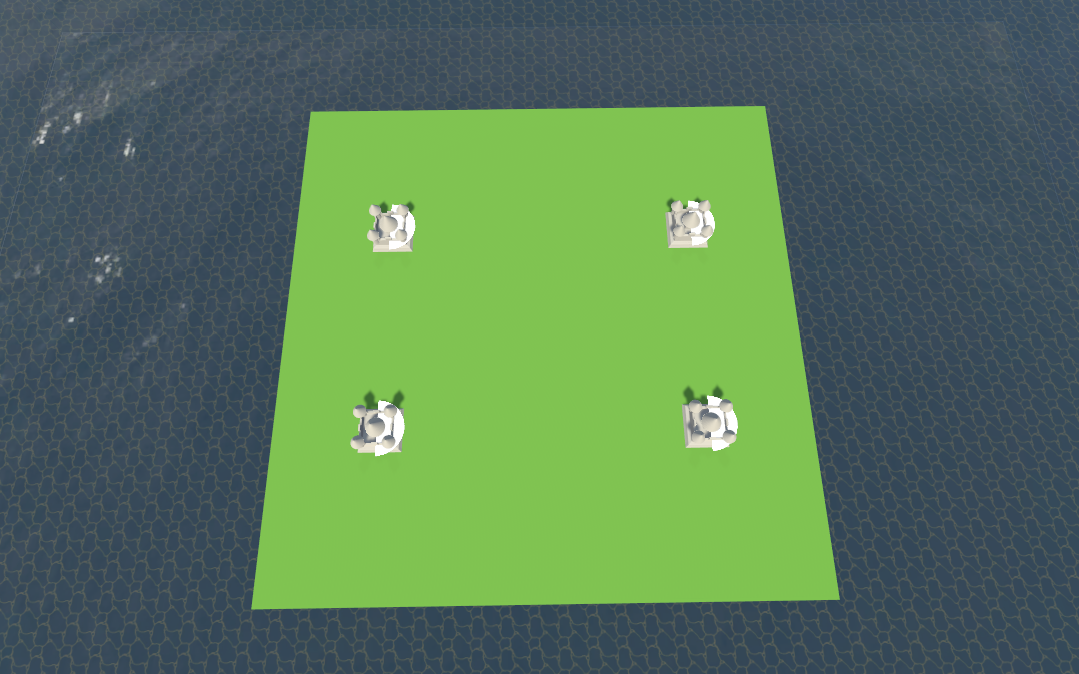
\includegraphics[scale=0.25]{MapSimpleImage}
        \caption{La carte Simple de Warbot.}
    \end{minipage}
    \hfill%
    \begin{minipage}[c]{.46\linewidth}
        \centering
        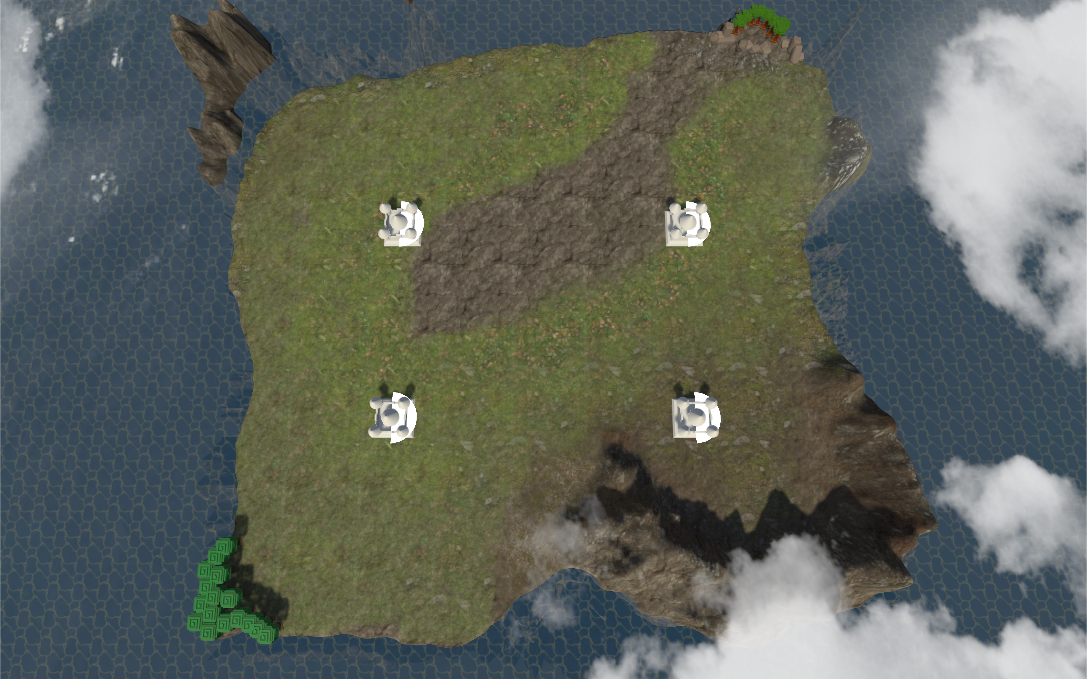
\includegraphics[scale=0.25]{MapMountainImage}
       \caption{La carte Mountain de Warbot.}
    \end{minipage}
\end{figure}
\begin{figure}[h]
    \begin{minipage}[c]{.46\linewidth}
        \centering
	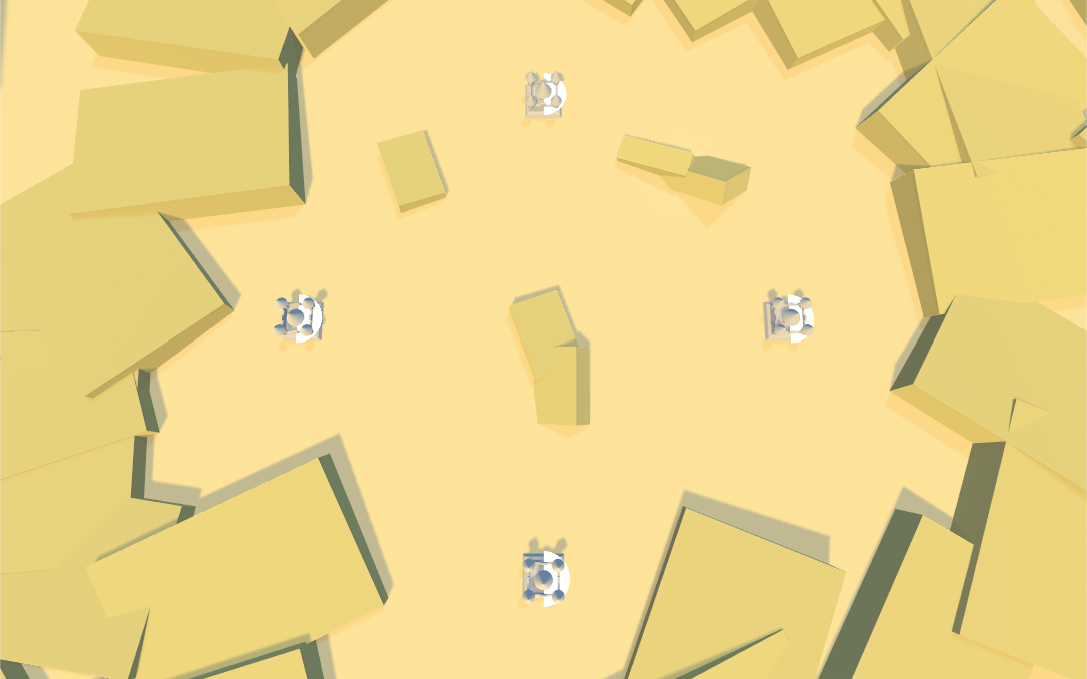
\includegraphics[scale=0.25]{MapDesolateImage}
	\caption{La carte Desolate de Warbot.}
    \end{minipage}
    \hfill%
    \begin{minipage}[c]{.46\linewidth}
        \centering
	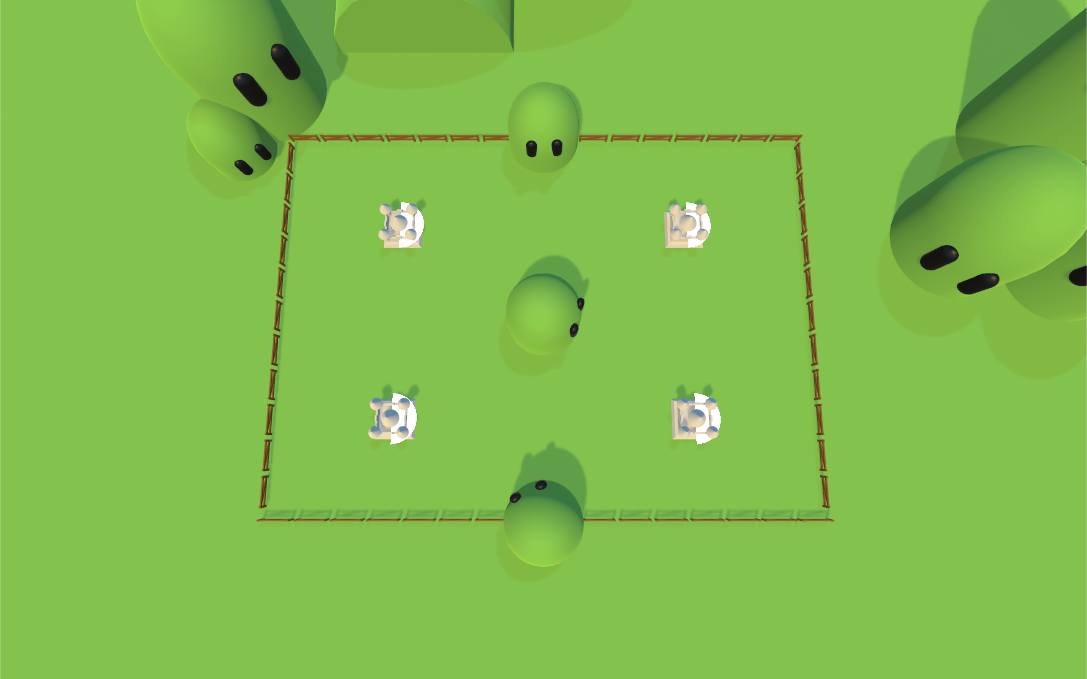
\includegraphics[scale=0.25]{MapPlainImage}
	\caption{La carte Plain de Warbot.}
    \end{minipage}
\end{figure}
\begin{figure}[!h]
        \centering
		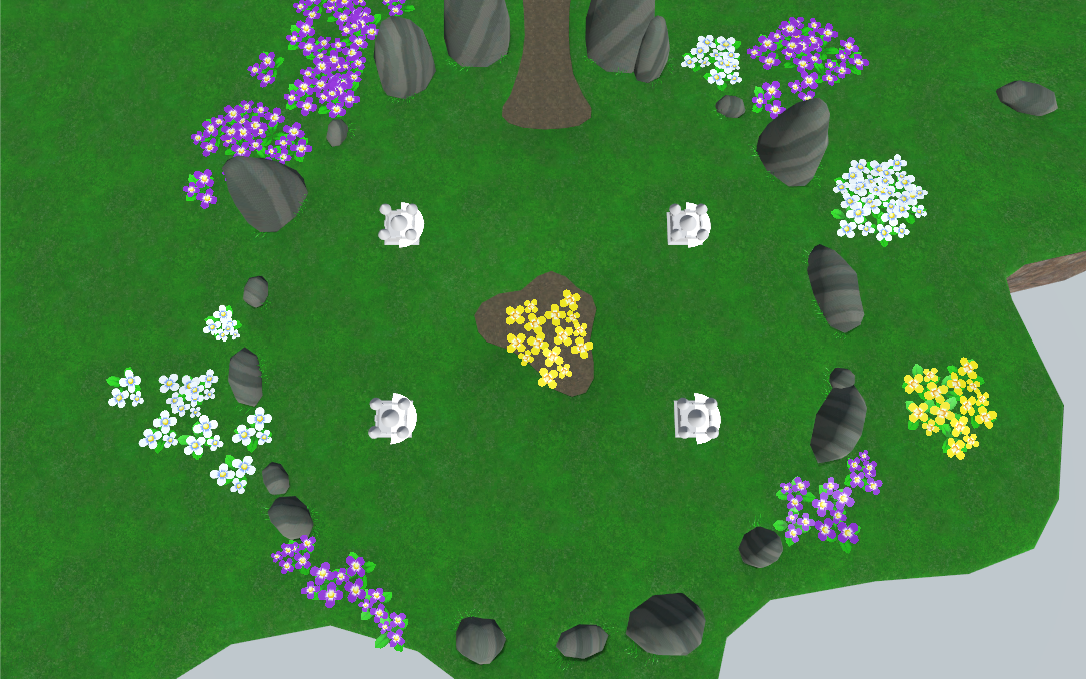
\includegraphics[scale=0.25]{MapGardenImage}
	\caption{La carte Garden de Warbot.}
\end{figure}
\newpage
\newpage
\newpage
\newpage


\subsection{Animations.}
Différentes animations ont été réalisées à l'aide de systèmes à particules afin d'améliorer le rendu visuel durant les combats entre unités.
\paragraph{Les projectiles.}
Au moment de la destruction d'un projectile, qui intervient lorsque celui-ci touche une unité ou après un laps de temps suivant son lancement, celui-ci provoque une explosion de particules. Les Prefab "HeavyBullet" et "LightBullet" possède pour ce faire un script "BulletScript.cs". Celui-ci instancie le GameObject d'animation correspondant au projectile au moment souhaité. Ce GameObject peut bien sûr être modifier facilement.
\paragraph{Les unités.}
Les autres animations concernent les unités qui détiennent toutes quatre animations différentes :
\begin{itemize}
\item L'unité se met à fumer légèrement lorsque ses points de vie sont entre 75\% et 100\%.
\item Une fumée plus épaisse se déclenche lorsque ses points de vie sont entre 50\% et 75\%.
\item L'unité est en feu lorsque ses points de vie sont entre 25\% et 50\%.
\item Pour finir elle explose en un amas de particule lorsque ses points de vies atteignent 0.
Les GameObject concernant ces différentes animations sont présents au sein des statistiques de chaque unité et peuvent être remplacés simplement.
\end{itemize}
 \begin{lstlisting}[language={[Sharp]C},label={lst:statsAnimation}, caption= Extrait du code de Stats.cs]
    [Header("Effects")]
    public GameObject _smallSmoke;
    public GameObject _largeSmoke;
    public GameObject _fire;
    public GameObject _explosion;

    private GameObject _currentEffect;
    void Start()
    {
        [...]
        _smallSmoke.SetActive(true);
        _largeSmoke.SetActive(true);
        _fire.SetActive(true);
        _explosion.SetActive(true);
    }
 [...]
void SetSmoke()
    {
        if (_currentEffect)
        {
            
        }
        if (_health > _maxHealth * 0.75)
        {
            Destroy(_currentEffect);
        }
        else if (_health > _maxHealth * 0.50)
        {
            if (_currentEffect)
            {
                Destroy(_currentEffect);
            }
            _currentEffect = Instantiate(_smallSmoke, transform.position, Quaternion.identity);
        }
        else if (_health > _maxHealth * 0.25)
        {
            if (_currentEffect)
            {
                Destroy(_currentEffect);
            }
            _currentEffect = Instantiate(_largeSmoke, transform.position, Quaternion.identity);
        }
        else if (_health > 0)
        {
            if (_currentEffect)
            {
                Destroy(_currentEffect);
            }
            _currentEffect = Instantiate(_fire, transform.position, Quaternion.identity);
        }
    }
\end{lstlisting}
\paragraph{Spécificité de unités de type Light.} La particularité de ceux-ci est qu'ils ont une tourelle rotative. Elle s'aligne en direction en direction de l'ennemi avant de tirer, cette caractéristique est particulièrement appréciable en mode de caméra première personne.
 \begin{lstlisting}[language={[Sharp]C},label={lst:ShooterAnimation}, caption= Extrait du code de Shooter.cs]
public void Shoot()
    {
        if (reloadTick == 0)
        {
            GameObject weapon = Instantiate(_weapon);
            _i = (_i + 1) % _listOfStartPoint.Length;
            weapon.transform.position = _listOfStartPoint[_i].position;
            weapon.GetComponent<BulletScript>()._owner = gameObject;
            Transform canon = null;
            for (int i = 0; i < transform.childCount - 1; i++)
            {
                if (transform.GetChild(i).transform.CompareTag("Canon"))
                {
                    canon = transform.GetChild(i);
                }
            }


            //If the child was found.
            if (canon != null)
            {
                weapon.GetComponent<BulletScript>()._vect = -canon.right;
            }
            else weapon.GetComponent<BulletScript>()._vect = Utility.vectorFromAngle(GetComponent<Stats>().GetHeading());
            reloadTick = GetComponent<Stats>().GetReloadTime();
        }
    }
\end{lstlisting}
\subsection{Sons.}
Les différents sons et bruitages présents dans le jeu ont été récupérés à partir de banques de sons libres de droit sur internet.
\newline Différents fonds musicaux et effets sonores sont audibles tout au long de l'utilisation du jeu.
\paragraph{Fonctionnement.}
Pour utiliser le son dans le moteur de jeu Unity, il faut passer par deux composants :
\begin{itemize}
\item Audiosource : un AudioSource est attaché a un GameObject pour lire les sons dans un environnement 3D, on peut lire un seul clip audio en utilisant Lecture, Pause et Stop. On peut également ajuster son volume pendant la lecture en utilisant la propriété de volume (expliqué plus en détail dans la partie Interface Graphique). Plusieurs sons peuvent être lus sur une source audio en utilisant PlayOneShot.
\item AudioListener :un AudioListener agit comme un périphérique de type microphone. Il reçoit une entrée de n'importe quelle AudioSource dans la scène et joue des sons à travers les haut-parleurs de l'ordinateur. Pour la plupart des applications, il est plus logique d'attacher l'AudioListener à la caméra principale. Il ne peut y avoir qu'un seul AudioListener par scène.
\end{itemize}
\paragraph{Les fond sonores.}
Deux ambiances musicales sont proposés sur l'ensemble du jeu.
\newline La première est activée dès le démarrage du jeu. Elle est jouée en boucle sur l'écran principal ainsi que sur l'éditeur sans interruption au passage de scène en scène.
\newline  La seconde est la musique en cours de jeu, elle démarre à chaque nouveau lancement de partie et est elle aussi jouée en boucle.
\newline Pour ce faire, le composant AudioSource utilisé est attaché au GameManager dont le script "GameManager.cs" a en attribut les deux AudioClip correspondant aux fonds sonores. Un AudioClip contient les données audio utilisées par un AudioSource.
 \begin{lstlisting}[language={[Sharp]C},label={lst:GameManagerSound}, caption= Extrait du code de GameManager.cs]
    public AudioClip audioMenu;
    public AudioClip audioWarbot;
\end{lstlisting}
Ci-dessous un exemple de changement de piste audio par appuie sur le bouton "Quit" sur l'écran de jeu. La piste audio correspondant aux menu est jouée.
\begin{lstlisting}[language={[Sharp]C},label={lst:HUDmanagerQuit}, caption= Extrait du code de HUDmanager.cs ]
    public void QuitToMenu()
    {
        SceneManager.LoadScene(0);
        audioSource.clip = gameManager.GetComponent<GameManager>().audioMenu;
        audioSource.Play();
    }
\end{lstlisting}
\paragraph{Les projectiles.}
Les deux projectiles, celui lancé par les chars légers et par les chars lourd produisent des sons lors de leur création et de leur destruction.
Ils ont chacun leur propre duo de sons et utilise l'AudioSource du GameManager pour les jouer. Comme se sont des sont ponctuels, on utilise la fonction PlayOneShot de l'AudioSource afin de les jouer.
\begin{lstlisting}[language={[Sharp]C},label={lst:bulletAudio}, caption= Extrait du code de BulletScript.cs ]
    public AudioClip _shotSongStart;
    public AudioClip _shotSongFinish;
    AudioSource audioSource;
    void Start()
    {
        audioSource = GameObject.Find("GameManager").GetComponent<AudioSource>();
        if (_shotSongStart != null) audioSource.PlayOneShot(_shotSongStart);
    }
\end{lstlisting}
\paragraph{Les unités.}
Chaque unité a un son correspondant à sa destruction, ceux-ci sont donc jouer à la mort de l'unité. Ces sons sont gérés de manière identique à celle utilisée pour les projectiles. Leurs lecture se fait dans le script "Stats.cs", en même temps que la mise à jour des points de vies. 
\begin{lstlisting}[language={[Sharp]C},label={lst:bulletAudio}, caption= Extrait du code de Stats.cs ]
if (_health <= 0)
        {
            if (_currentEffect)
            {
                Destroy(_currentEffect);
            }
            _currentEffect = Instantiate(_explosion, transform.position, Quaternion.identity);
            if (_dieSong != null) audioSource.PlayOneShot(_dieSong);
            Destroy(_currentEffect, 1.5f);
            Destroy(gameObject);
        }
\end{lstlisting}
\section{Améliorations possibles}
L’objectif de ce projet était de rendre générique la version Warbot Unity réalisée l'an dernier.
Le but étant de facilité la création sur le moteur de jeu Unity, de jeux de stratégie basés sur le paradigme de  la programmation orientée agent afin de permettre un véritable apprentissage de ses différentes notions. Mais les corrections et améliorations possibles pour les années à
venir sont multiples :
\begin{itemize}
\item Corriger le problème provoquant la rotation des bases lors de la transmission de message..
\item Corriger le positionnement sur l'axe z des unités.
\item Perfectionner la gestion des collisions des unités.
\item Améliorer les modèles 3D.
\item Créer de nouveaux percepts, de nouvelles actions terminales et non terminales.
\item Ajouter la possibilité de créer, supprimer et déplacer des unités directement en jeu.
\item Intégrer la notion de groupe au comportement des unités.
\item Permettre la sauvegarde d'une partie en cours de jeu et la reprise de celle-ci ultérieurement.
\item Permettre la création de comportements sous forme de machine à état finie en plus de l'architecture de subsomption actuellement présente.
\item Permettre la désactivation/activation du Friendly Fire actuellement non désactivable.
\item Rendre fonctionnel l'application sur Mac et Android.
\item De manière générale corriger l'ensemble des bugs présents dans la partie dédiée.
\item Optimiser le moteur de jeu.
\end{itemize}

\newpage
%%%
% PARTIE Interface Graphique
%%%
\chapter{Partie Interface Graphique}
\section{Présentation}
La partie Interface Graphique fait le lien entre l'utilisateur, et toutes les fonctionnalités existantes dans le moteur. Elle comprend principalement l'habillage visuel des éléments avec lequel l'utilisateur va interagir pour jouer au jeu. MetaBot étant un jeu pour "programmeur", le joueur interagit surtout avec le menu principal et l'éditeur de comportement, afin de créer des équipes pour pouvoir les faire s'affronter. \newline


\section{Etude de l'ancienne interface}
L'ancienne interface, sur laquelle nous avons du baser notre travail, se décomposait en trois parties.
\begin{itemize}
\item\textbf{Le menu principal}
\item\textbf{L'éditeur de comportement}
\item\textbf{La sélection d'équipes}
\end{itemize}
\subsection{Menu Principal}
Le menu principal, à première vue, est assez classique. Quatre options s'offrent à nous :
\begin{itemize}
\item{Lancer une nouvelle partie}
\item{Accéder à l'éditeur de comportement}
\item{Quitter le jeu}
\item{Activer / Désactiver le son}
\end{itemize}
L'aspect purement graphique est cohérent, puisque le fond d'écran représente une scène de jeu.
Nous pouvons donc apercevoir deux modèles 3D d'unités présentes en jeu, ainsi qu'une partie du décor sur mequel se déroulera le combat.

\begin{figure}[!h]
	\centering
		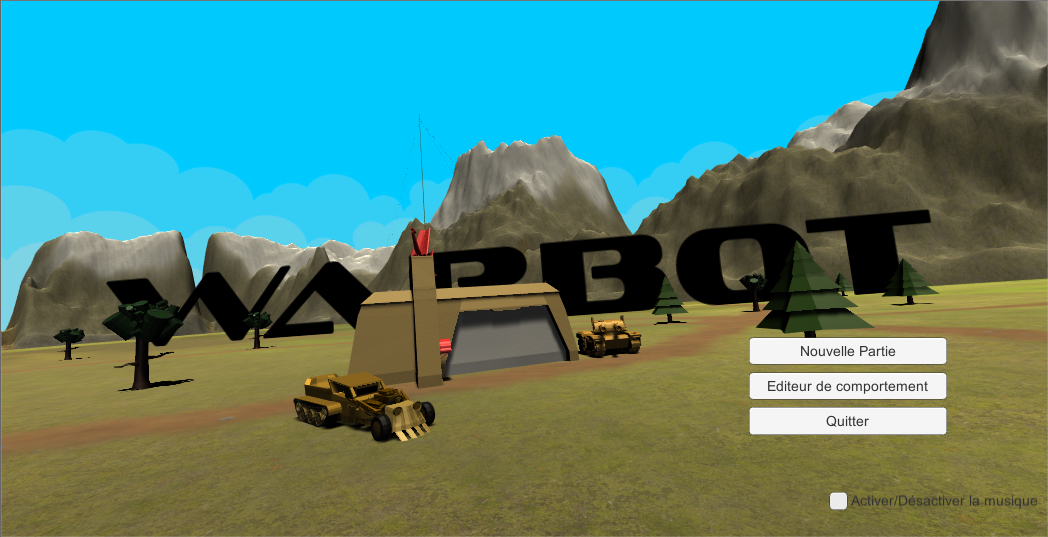
\includegraphics[scale=0.50]{MainScreenOld}
	\caption{Menu Principal, Ancienne Interface}
\end{figure}

\subsection{Editeur de comportement}
L'éditeur de comportement se décompose en deux écrans distincts  : 
\begin{enumerate}
\item\textbf{Le menu Pause}
\paragraph{}
Ce menu apparaît par défaut lors d'une tentative d'accès à l'éditeur de comportement si aucune équipe n'existe. Il permet donc de créer une nouvelle équipe, en entrant son nom.\newline
De plus, il permet de revenir au menu principal, de lancer une nouvelle partie, de quitter le jeu, ou bien tout simplement de fermer ce menu pour accéder à l'éditeur de comportement.\newline
Ce menu est toutefois "caché". Pour y accéder, il faut appuyer sur la touche "ECHAP" du clavier pour le voir s'afficher.
\clearpage
\begin{figure}[h]
	\centering
		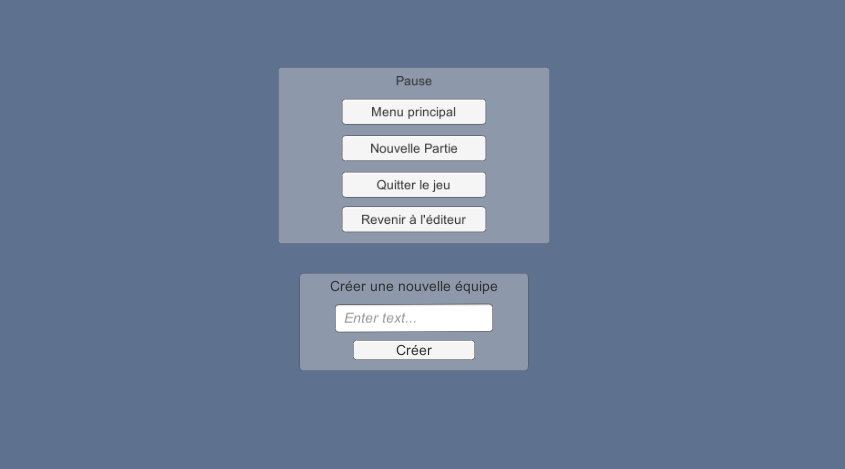
\includegraphics[scale=0.50]{PauseMenuOld}
	\caption{Menu Pause, Ancienne Interface}
\end{figure}


\item\textbf{L'éditeur en lui même}\newline
Nous avons maintenant devant nous un éditeur sobre. En haut à gauche se trouve le nom de l'équipe courante, ainsi que l’unité sur laquelle on va travailler.\newline
Juste en dessous, une liste de primitives, utiles à la création de comportement.\newline
Et enfin, à droite, la zone d'édition.

\begin{figure}[h]
	\centering
		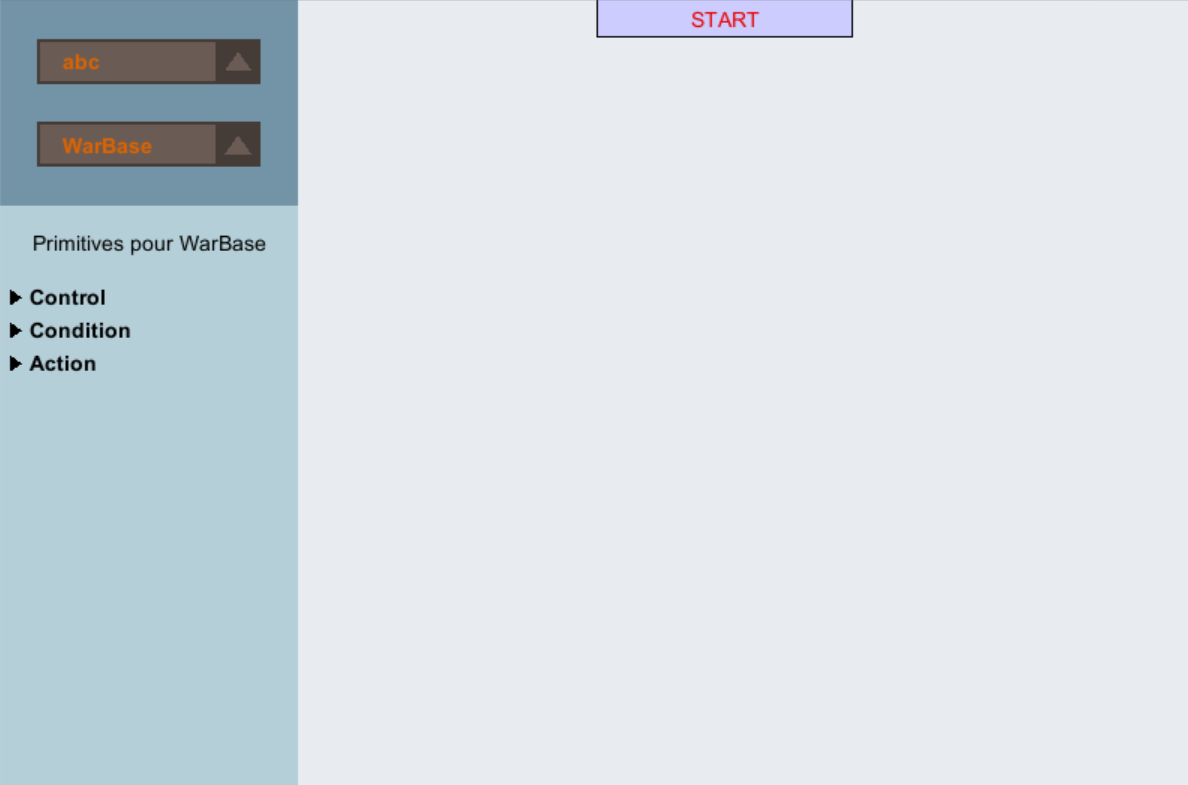
\includegraphics[scale=0.50]{BehaviorScreenOld}
	\caption{Editeur de Comportement, Ancienne Interface}
\end{figure}

\end{enumerate}


\subsection{La séléction des équipes}
Une fois le bouton "Nouvelle partie" cliqué, nous arrivons sur un nouvel écran, permettant de choisir les équipes qui vont participer, ainsi que le nombre de chacune de leurs unités qui commenceront directement en jeu.\newline
Cet écran permet également de revenir au menu principal, ou bien tout simplement de lancer la partie. Cette étape supplémentaire demandé à l'utilisateur ne nous paraissait pas spécialement utile. L'écran ne propose rien d'autre que la gestion des paramètres de partie. L'espace utilisé est moindre pour justifier l'affichage d'un nouvel écran.

\begin{figure}[!h]
	\centering
		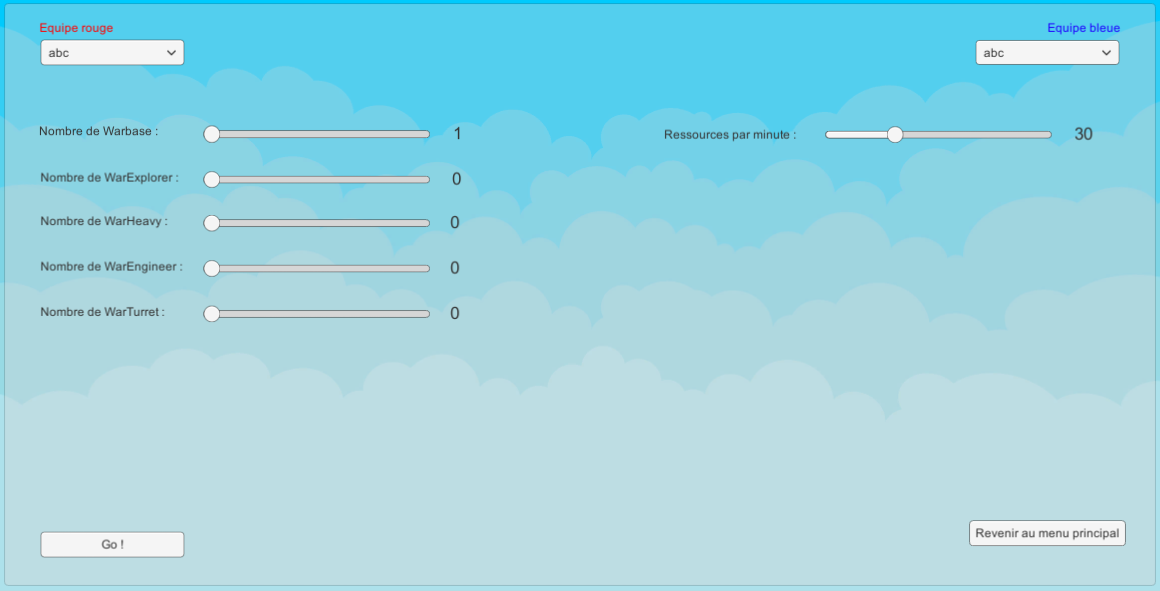
\includegraphics[scale=0.50]{SettingsOld}
	\caption{Sélection des équipes, Ancienne Interface}
\end{figure}

\subsection{Améliorations envisagées}
\paragraph{}
Les fonctionnalités primordiales au bon fonctionnement du jeu sont disponibles :
\begin{itemize}
\item La sélection de l’équipe et de toutes les unités 
\item La liste des primitives concernant l’unité sélectionnée 
\item La description et le placement des primitives 
\item La création et l’édition de l’architecture de subsomption via l’aire de jeu
\end{itemize}

Ceci dit, nous souhaitions revoir quelques points. \newline
Premièrement, nous voulions que tout soit le plus intuitif possible pour l'utilisateur. Il fallait que toutes les fonctionnalités proposées soient accessibles facilement. Par exemple, la création d'équipe n'est pas évidente à trouver. Il faut passer par un menu "caché" (appuyer sur la touche "ESC" depuis l'éditeur de comportement) pour pouvoir y accéder. Nous voulions éviter ce genre de problèmes. Des petits soucis d'optimisations étaient également présents, tel que la difficulté d'aimanter deux blocs. Si on ne posait pas le bloc à un endroit précis, il disparaissait. Il fallait alors le sélectionner à nouveau dans la liste de primitives, et retenter l'opération. A force, cela peut vite devenir redondant.
\newline
\smallbreak
Bien que l'éditeur soit fonctionnel, il nous paraissait assez austère, pas suffisamment "User Friendly". L'utilisateur passe la majeur partie de son temps sur cet écran. Il fallait donc qu'il soit le plus agréable  possible à l’œil, pour ne pas lasser l'utilisateur, et lui donner envie de passer du temps dessus.\newline \smallbreak
Enfin, l'absence totale de paramètres nous a semblé dommage. On ne peut qu'activer ou désactiver le son, mais pas régler le volume. L'utilisateur ne sait pas comment gérer les équipes qui vont participer, ainsi que leur nombre d'unités, avant d'avoir cliqué sur Nouvelle Partie. Ce comportement ne parait pas intuitif. L'ajout d'une gestion des paramètres nous semblait donc indispensable.

Nous avons donc décidés de revoir l'organisation de l'interface depuis le début. Adapter cette interface n'aurait pas été justifié, car trop de changements étaient à prévoir, tant sur le point technique que graphique.\newline
Nous souhaitions également proposer une cohésion graphique entre chaque écran, et le jeu lui-même.


\section{Nouvelle Interface}
Nous devions repartir d'une toute nouvelle interface, tout en s'inspirant de l'ancienne. Comme dit précédemment, nous voulions éviter au maximum les écrans intermédiaires qui n'étaient pas indispensables.
Nous avons donc décidé de mettre en place deux écrans : le menu principal,  et l'éditeur de comportement. Dans le menu principal se trouve une fenêtre "pop-up" dédiée à la configuration des paramètres. D'autres fenêtres "pop-up" peuvent apparaître, mais elles n'ont que pour but d'effectuer une vérification de l'action émise par l'utilisateur. Par exemple, confirmer la suppression d'une équipe, confirmer la fermeture du jeu, etc...

\subsection{Menu Principal}
Le menu principal donne accès aux options majeures du jeu. Ce menu doit contenir toutes les fonctionnalités dont l'utilisateur peut avoir besoin pour gérer le lancement d'une partie, sans avoir à accéder à l'éditeur de comportement.
Cela comporte donc les paramètres de la partie, le choix des équipes, du nombre d'unités, de la carte, etc... \newline
\begin{figure}[!h]
	\centering
		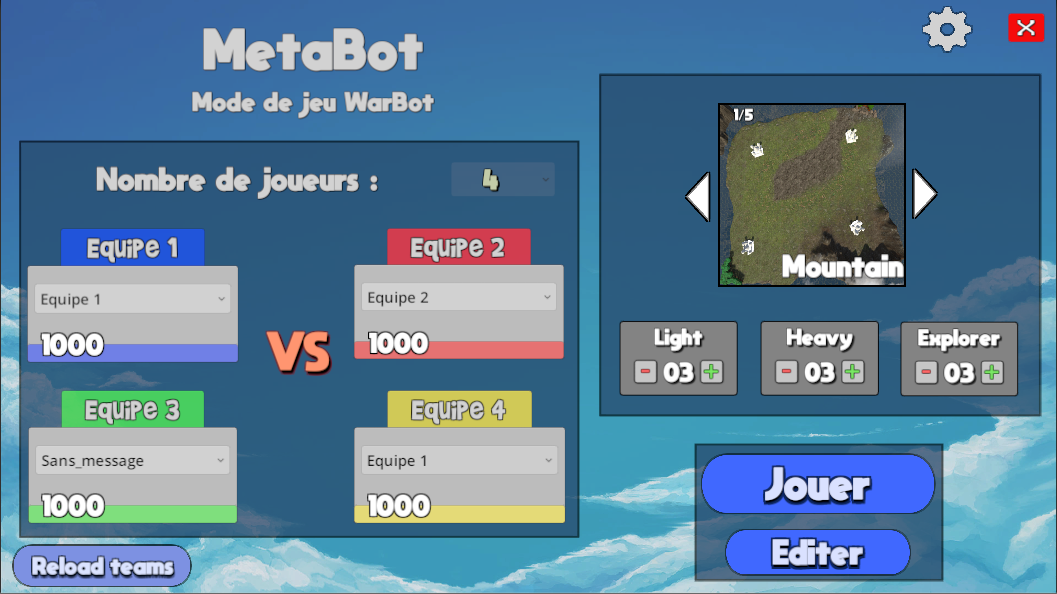
\includegraphics[scale=0.50]{MenuPrincipal}
	\caption{Menu Principal, Nouvelle Interface}
\end{figure}
Passons en revue tous les éléments présents sur cet écran.
\subsubsection{Lancer une Partie}
Le bouton "Jouer" permet de lancer une partie du jeu MetaBot. Le lancement de la partie prend en compte le mode de jeu sélectionné, les équipes choisies, le nombre de chaque unités en début de partie, le nombre de ressources maximum (nombre de ressource présentes en jeu au même moment), et la carte de jeu. Un script rattaché à ce bouton va donc se charger d'aller récupérer toutes ces informations stockées dans les différents "GameObject" de notre scène.

\begin{lstlisting}[language={[Sharp]C},label={lst:StartGame()}, caption= Extrait du code de PlayButton.cs]

public void StartGame()
    {
        
        nbPlayers = int.Parse(_numberplayerDropDown.GetComponent<Dropdown>().captionText.text);
        XMLWarbotInterpreter interpreter = new XMLWarbotInterpreter();

        GameObject gameManager = GameObject.Find("GameManager");
        string gamePath = Application.streamingAssetsPath + "/teams/" + gameManager.GetComponent<GameManager>()._gameName + "/";
        
        gameManager.GetComponent<TeamManager>()._teams = new List<Team>();

        for (int i = 0; i < nbPlayers; i++)
        {
            Team team = new Team();
            team._color = _DropDownList[i]._teamColor;
            team._name = _DropDownList[i]._teamName;//.Replace("_", " ");
            team._unitsBehaviour = interpreter.xmlToBehavior(gamePath + team._name, gamePath);
            gameManager.GetComponent<TeamManager>()._teams.Add(team);
        }

        GameManager setting = gameManager.GetComponent<GameManager>();
        setting.SetSetting();

        //
        StartCoroutine(AsynchronousLoad(setting._gameSettings._indexSceneMap));
    }
}
\end{lstlisting}


\subsubsection{Bouton Éditeur de Comportement}
Le bouton "Editer" permet d'accéder à l'éditeur de comportement, qui permettra à l'utilisateur, entre autres, de créer et/ou modifier le comportement de ses équipes.
\subsubsection{Bouton Paramètres}
L'icône en forme d'engrenage représente le bouton paramètres. Il va permettre d'afficher la fenêtre "pop-up" qui contient tous les paramètres du jeu.
\subsubsection{Choisir le nombre d'équipe}
Nous avons la possibilité de choisir le nombre d'équipes participant à la partie. Les valeurs sont dans un menu déroulant et vont de 2 à 4. Sa valeur courante sera récupérée par le script StartGame() (cf Listing 4.1).\newline
En fonction du nombre d'équipes choisies, le nombre de cadres d'équipe changera.
\subsubsection{Choisir les équipes}
Dans le cadre de chaque équipe se trouve un menu déroulant avec les noms de toutes les équipes présentes dans les fichiers du jeu. On peut donc en sélectionner une pour qu'elle participe à la prochaine bataille.
Pour récupérer toutes les équipes existantes, nous allons chercher la liste comprenant le nom de toutes les équipes.

\begin{lstlisting}[language={[Sharp]C},label={lst:Start()}, caption= Extrait du code de TeamMenuHUD.cs]
[...]
string team = GameObject.Find("GameManager").GetComponent<TeamManager>()._teams[_idPlayer]._name;
            for (int i = 0; i < _teamDropDown.options.Count; i ++)
            {
                if (_teamDropDown.options[i].text.Equals(team))
                {
                    _teamDropDown.value = i;
                }
            }
[...]
\end{lstlisting}
\smallbreak
De plus, à coté du nom de l'équipe, on retrouve aussi son score (ELO). Pour son affichage, nous récupérons le score associé à l'équipe courante. La couleur du score dépendra de sa valeur. (rouge = score faible, bleu = score élevé)

\begin{lstlisting}[language={[Sharp]C},label={lst:Change()}, caption= Extrait du code de TeamMenuHUD.cs]
public void Change()
    {
        _teamName = _teamDropDown.captionText.text;
        _powerScoreText.text = TeamsPerformance.GetTeamElo(_teamName).ToString();
        _powerScoreText.color = ColorElo(TeamsPerformance.GetTeamElo(_teamName));
    }
\end{lstlisting}
\subsubsection{Bouton "Reload Team"}
Ce bouton permet de recharger les équipes. L'intérêt est de permettre à l'utilisateur d'ajouter manuellement au dossier des équipes des nouveaux fichiers d'équipes, et de les voir apparaître en cliquant simplement sur ce bouton, sans avoir à relancer le jeu.
Pour permettre cela, nous devons aller chercher le dossier contenant les fichiers des équipes, le parcourir, et mettre à jour notre liste d'équipes.

\begin{lstlisting}[language={[Sharp]C},label={lst:Updating()}, caption= Extrait du code de GameSettingsScript.cs]
teams = new List<string>();
        string[] fileEntries = Directory.GetFiles(gamePath);
        foreach (string s in fileEntries)
        {
            string team = stringDifference(s, gamePath);
            if (team.Contains(".wbt") && !team.Contains(".meta"))
            {
                teams.Add(team);
            }
        }
\end{lstlisting}

\subsubsection{Choisir carte de jeu}
On peut directement choisir le lieu de la partie en cliquant sur les flèches de part et d'autre de l’aperçu de la carte. Il existe pour le moment cinq cartes: Moutain, Plain, Simple, Desolate et Garden. Chaque changement de carte mettra à jour le nom affiché, ainsi que le visuel de l'aperçu de la carte. Pour cela, il suffit de récupérer le nom de la carte sélectionnée, ainsi que son visuel associé, puis de les afficher.

\begin{figure}[!h]
	\centering
		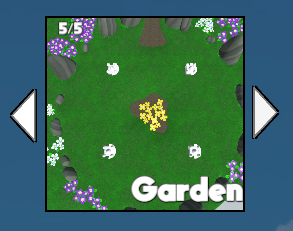
\includegraphics[scale=0.80]{ChoiceMap}
	\caption{Aperçu de la sélection de carte}
\end{figure}
\subsubsection{Choisir nombre de départ de chaque unité}
En dessous de l’aperçu de la carte, il y a les noms des unités existantes. Sous ces noms, le chiffre indique le nombre de ce type d'unité présent au lancement de la partie. On peut incrémenter ou décrémenter ce chiffre à l'aide des boutons "+" et "-" à coté de celui-ci. A chaque clic sur le bouton "+", on incrémente la variable "number" associée à l'unité, et inversement avec "-", dans la limite du possible ( c'est-à-dire tout en vérifiant que la valeur maximale du nombre d'unités possible ne soit pas dépassé).

\begin{lstlisting}[language={[Sharp]C},label={lst:Add()}, caption= Extrait du code de UnitSettingMenu.cs]
_number = Mathf.Min(_maxNumber, _number + 1);
_unitCounter.text = _number.ToString("00");
\end{lstlisting}

\begin{figure}[!h]
	\centering
		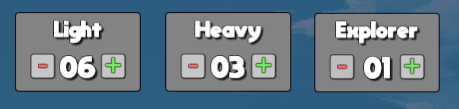
\includegraphics[scale=0.80]{NumberUnits}
	\caption{Choix du nombre d'unités}
\end{figure}

\subsubsection{Barre de Chargement}
Quand on lance une partie, une barre de chargement apparaît et indique l'avancement du chargement de la partie.
Ceci est une fonction qui utilise "AsyncOperation". La variable ao va contrôler l'avancée du chargement de la scène jeu.
Nous allons récupérer cette valeur, et la passer à notre slider.
La scène se chargera qu'une fois la progression de l'AsyncOperation terminée.
De cette manière, l'utilisateur peut voir où en est le chargement de sa partie.

\begin{lstlisting}[language={[Sharp]C},label={lst:Add()}, caption= Extrait du code de UnitSettingMenu.cs]
IEnumerator AsynchronousLoad(int scene)
    {
        loadingScreenBar.SetActive(true);
        yield return null;
        AsyncOperation ao = SceneManager.LoadSceneAsync(scene);
        ao.allowSceneActivation = false;
        while (!ao.isDone)
        {
            sliderLoad.value = ao.progress;
            if (ao.progress == 0.9f)
            { 
               sliderLoad.value = 1f;
               ao.allowSceneActivation = true;
            }
            yield return null;
        }
    }
\end{lstlisting}

\subsubsection{Bouton Quitter}
Ce bouton ouvre une boite de dialogue demandant à l'utilisateur s'il veut vraiment quitter le jeu. Il peut ainsi choisir de revenir sur le menu principal ou fermer le jeu.

\subsection{Menu des Paramètres}
Ce menu regroupe tous les paramètres modifiables par l'utilisateur. En ouvrant cette fenêtre, l'utilisateur aura donc la possibilité de personnaliser son expérience de jeu, en modifiant les valeurs des paramètres. Cela permet de renouveler la dynamique des parties, et d'offrir une expérience nouvelle. \newline
\smallbreak
Au delà des paramètres concernant directement le déroulement de la partie, l'utilisateur peut également modifier la langue du jeu. L'utilisateur peut alors choisir la langue avec laquelle il est le plus à l'aise.
\begin{figure}[h]
	\centering
		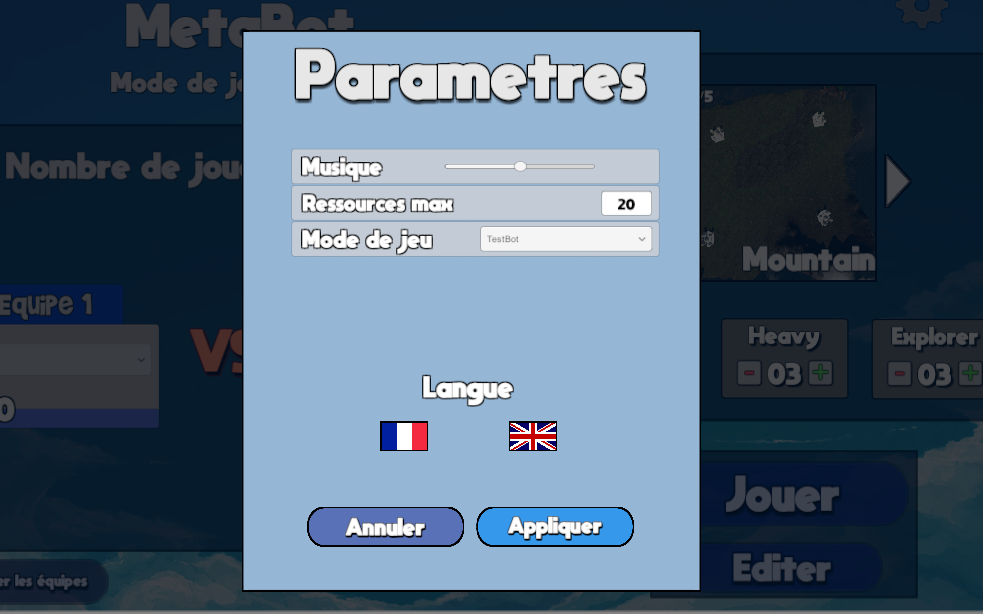
\includegraphics[scale=0.60]{MenuParametres}
	\caption{Fenêtre des paramètres}
\end{figure}

\subsubsection{Choisir le nombre de ressource maximales dans le jeu}
Dans cette case, on peut entrer un chiffre entier qui indiquera le nombre maximum de ressources présentes simultanément en jeu.
\begin{figure}[h]
	\centering
		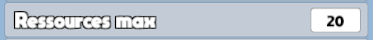
\includegraphics[scale=0.80]{RessourcesMax}
	\caption{Choix du nombre maximal de ressources}
\end{figure}
\subsubsection{Choisir le mode de jeu}
Ce menu déroulant permet de choisir le mode de jeu de la prochaine partie. Il y a actuellement deux modes, le mode MetaBot et le mode RessourceRace. Le mode MetaBot est le mode classique. Le mode RessourceRace est une course aux ressources. La première équipe à atteindre le nombre de ressources fixé par le joueur gagne.

Si le mode choisi est RessourceRace alors deux autres paramètres apparaissent:
\begin{itemize}
\item le temps imparti
\item le nombre de ressources à atteindre pour gagner.
\end{itemize}

\begin{figure}[!h]
	\centering
		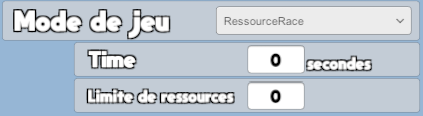
\includegraphics[scale=0.80]{ManuelJeu/ModeJeuRessourceRace}
	\caption{Paramètres RessourceRace}
\end{figure}

\subsubsection{Changer le volume de la musique}
Ce slider indique le niveau sonore de la musique. On peut le modifier en cliquant dessus et en déplaçant la valeur de 0 jusqu’à 100. 0 correspond à un arrêt de la musique et 100 au volume maximal. \newline
De plus, le volume sonore dans le menu est le même dans l'éditeur de comportement et dans le jeu lui même.
La valeur de notre slider affectera directement la valeur de notre AudioSource.
\smallbreak
\begin{figure}[h]
	\centering
		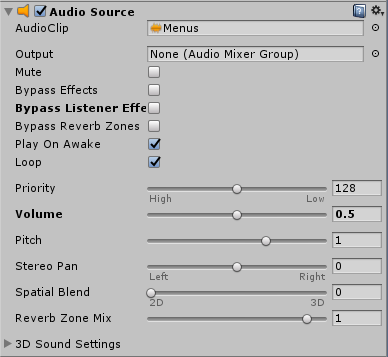
\includegraphics[scale=1]{AudioSource}
	\caption{Aperçu de l'AudioSource, dans l'Inspector}
\end{figure}

\subsubsection{Choisir la langue}
Les boutons en forme de drapeau indiquent les langues disponibles pour le jeu. Pour changer de langue, il suffit d'appuyer sur le drapeau voulu et de cliquer sur "Valider".
La traduction de chaque texte présent dans l'interface se fait grâce à des fichiers .yml, et .txt.
L'appel au traducteur permet ce changement. 
Nous ne traiterons pas en détail son fonctionnement, car il concèrne la partie Interpréteur.
\begin{lstlisting}[language={[Sharp]C},label={lst:ChangementLangue(string newLangage)}, caption= Extrait du code de ChangeLanguage.cs]
public void ChangementLangue(string newLangage)
    {
        GameObject.Find("GameManager").GetComponent<LangageLoader>().changeLanguage(newLangage);
        GameObject.Find("GameManager").GetComponent<Traducteur>().langue = newLangage;
        

        string[] lines = System.IO.File.ReadAllLines(Application.streamingAssetsPath+"/properties.yml");
        int cpt = 0;
        foreach (string line in lines)
        {
            if (line.Contains("Language"))
            {
                string[] tmp = line.Split('=');
                tmp[1] = newLangage;
                lines[cpt] = tmp[0] + "=" + tmp[1];
                break;
            }
            cpt++;
        }
        System.IO.File.WriteAllLines(Application.streamingAssetsPath+"/properties.yml", lines);
    }
\end{lstlisting}

\subsubsection{Bouton Retour}
Ce bouton permet de retourner à l'écran du menu principal.
Contrairement au bouton "Appliquer", ce bouton n'applique aucun changement effectué par l'utilisateur.

\subsubsection{Bouton Valider}
Ce bouton valide les paramètres définis précédemment et revient au menu principal en ayant appliqué ces paramètres.

\begin{lstlisting}[language={[Sharp]C},label={lst:ApplySettings()}, caption= Extrait du code de SettingsButton.cs]
public void ApplySettings()
    {
        setButtonActive();
        manageVolume();
        changeLanguage.ChangementLangue(language);
        changeGameMode();
        if(numberResources() == 0)
        {
            numberResources();
        }
        else
        {
            return;
        }
        window.SetActive(false);
    }
\end{lstlisting}

On peut apercevoir dans cette méthode, qu'elle appelle une méthode spécifique pour chaque paramètre modifiable.
Elle s'occupe donc d'appliquer chacune des modifications effectuées, via l'appel de la fonction adéquate.




\subsection{Editeur de Comportement}
\paragraph{}
Pour la refonte de l'éditeur de comportement, ce qui nous a paru le plus optimal fut de repartir d'une interface vierge. Nous avions identifié un nombre trop important de changements à effectuer pour justifier des modifications de l'ancienne interface.
Nous avons commencé par faire un croquis de deux interfaces potentielles.
\begin{figure}[!h]
	\centering
		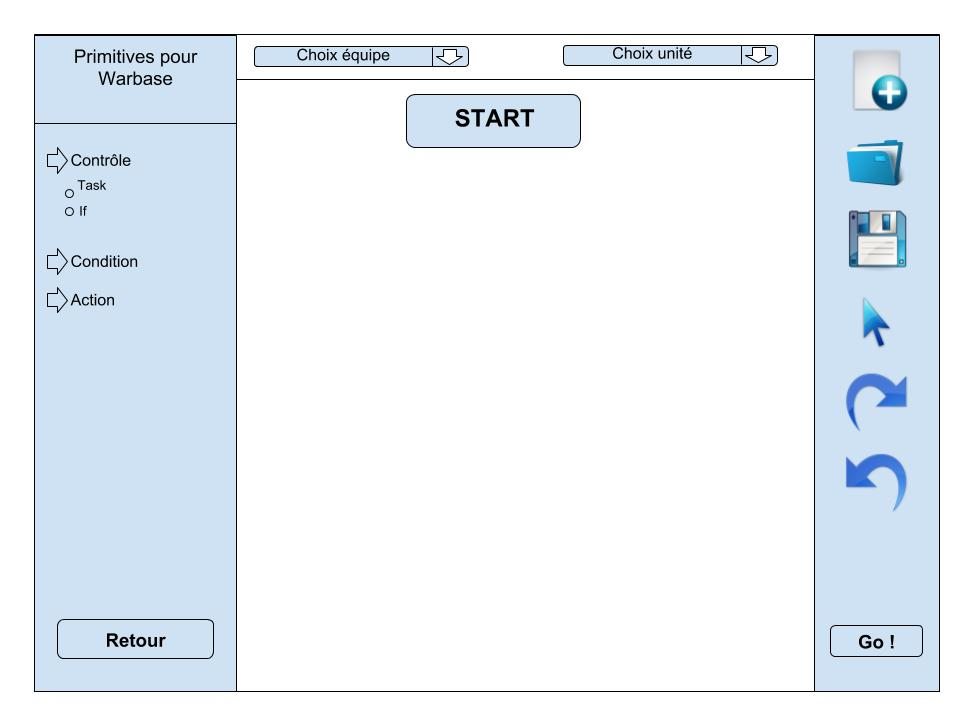
\includegraphics[scale=0.35]{ConceptionGraphique1}
	\caption{Première ébauche}
\end{figure}


\paragraph{}
Le premier modèle s'appuie sur l'esprit de l'ancienne interface, avec le panneau de contrôles fortement similaire. Cependant, après concertation lors d'une réunion, nous avons écarté ce modèle, car il ne semblait pas optimisé. La barre d'outils paraissait bien trop importante, et la zone d'édition de comportement s'en voyait restreinte.\clearpage
Quant au second modèle, il nous semblait organisé de manière plus logique, et intuitive. Toutes les options et choix se trouvent à gauche de la fenêtre, alors que la partie droite se consacre à l'édition du comportement.\newline
Nous avons donc décidé de partir sur ce modèle.

\begin{figure}[!h]
	\centering
		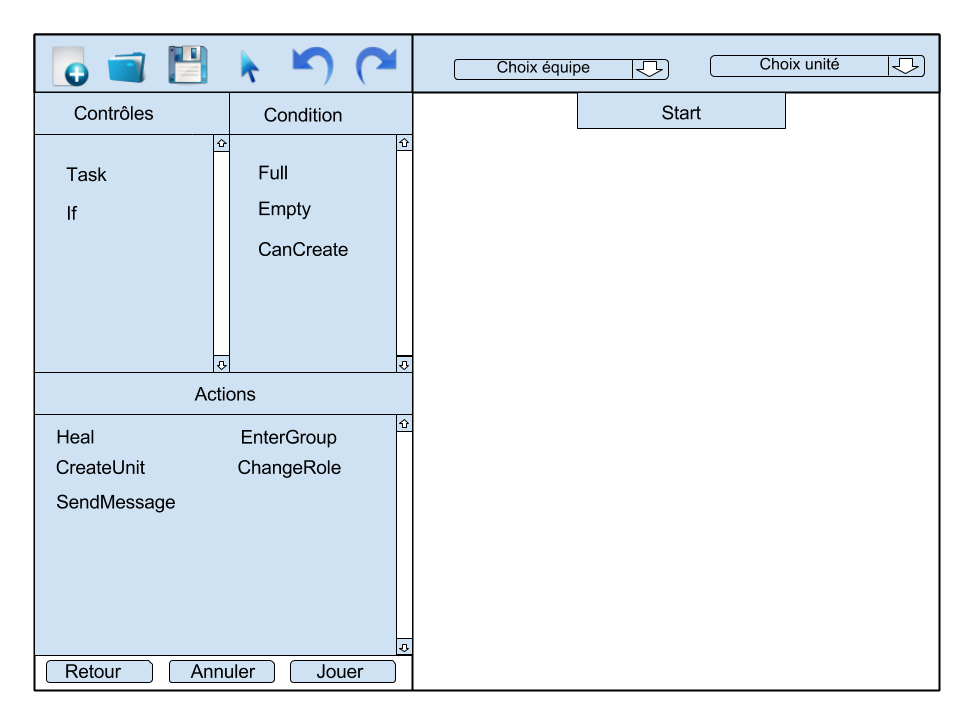
\includegraphics[scale=0.35]{ConceptionGraphique2}
	\caption{Seconde ébauche}
\end{figure}


\paragraph{}
Au fur et à mesure de nos avancées, de nouveaux éléments ont pris place dans l'interface. A force d'ajouter des informations et fonctionnalités, nous avons dû légèrement retravailler l'aspect global de l'écran, pour gagner en cohésion, et en ergonomie.
En voici un aperçu :
\clearpage
\begin{figure}[!h]
	\centering
		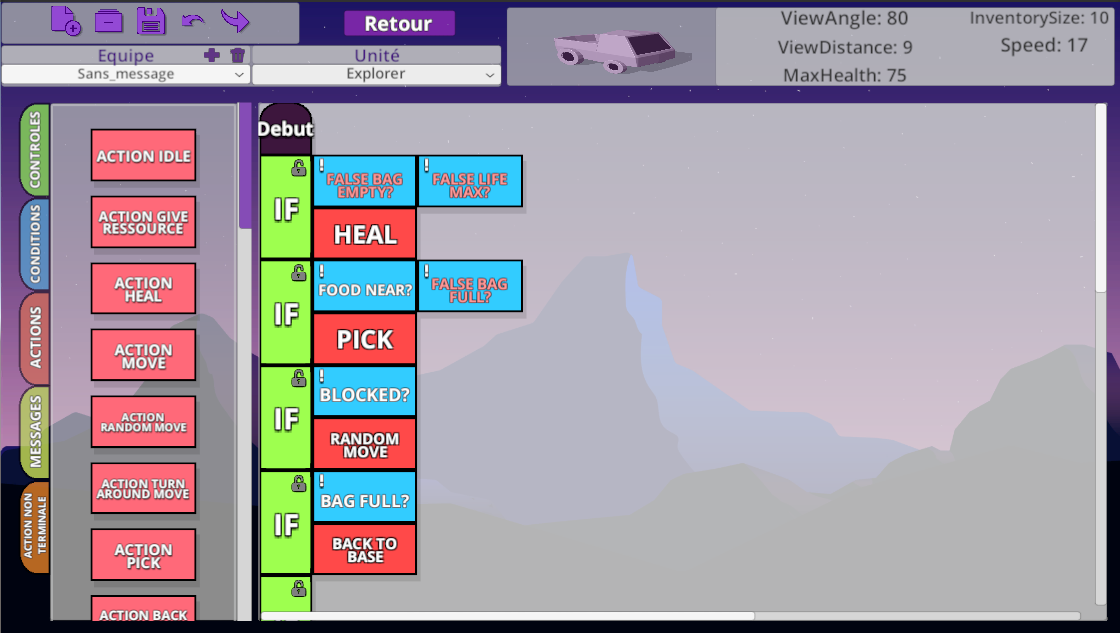
\includegraphics[scale=0.50]{InterfaceFinale}
	\caption{Interface Finale}
\end{figure}
% ToolBox %
\subsubsection{ToolBox}
La ToolBox est le panneau en haut à gauche de l'interface, regroupant des actions classiques, telles que la sauvegarde de fichier, la création d'un nouveau comportement, etc...

\begin{figure}[!h]
	\centering
		
\includegraphics[scale=0.50]{ToolBox}
	\caption{ToolBox, Editeur de comportement}
\end{figure}

\begin{enumerate}[label=\Alph*)]
\item\textbf{Bouton Nouveau Comportement} \newline
Ce bouton permet de commencer la création d'un nouveau comportement pour l'unité de l'équipe courante. Cela permet de repartir à zéro, lorsque notre comportement courant ne nous satisfait pas, et nous évite de devoir retirer chaque pièce manuellement.
\item\textbf{Bouton Chargement Comportement} \newline
Ce bouton permet de charger le comportement de l'unité actuellement sélectionnée dans le DropDown prévu à cet effet.
La première chose à faire est d'effacer le comportement actuellement chargé, s'il existe.
A l'aide du path, et du nom de l'équipe, nous allons pouvoir appeler une méthode présente dans l’interpréteur, pour transformer le fichier .xml correspondant à l'équipe courante, en un comportement, qui sera stocké dans un dictionnaire.\newline
Nous allons ensuite récupérer la position de la pièce "StartPuzzle", pour pouvoir placer les pièces correctement dans l'éditeur. Nous avons donc notre point de départ.\newline 
Il ne reste plus qu'à placer les pièces. Nous allons donc récupérer la liste d'instructions associée à chaque unité, et placer chaque instruction dans leur ordre d'apparition. (Un "if" pour commencer, suivi de sa ou ses conditions, suivies d'une ou plusieurs actions)\newline
Pour finir, on réinitialisera la scrollbar de l'éditeur, pour permettre à l'utilisateur de voir directement le début du comportement.\newline
\textit{Voir Annexes pour le script}
\item\textbf{Bouton Sauvegarde du Comportement} \newline
Ce bouton sauvegarde le comportement de l'unité de l'équipe courante. Si l'on change d'unité dans la même équipe sans sauvegarder, alors le comportement de l'unité précédente sera perdu.\newline
Voyons de plus près deux de ses fonctions primordiales au bon fonctionnement du script :

Nous allons créer un comportement, copiant le comportement présent dans l'éditeur. Pour commencer, nous allons répertorier toutes les pièces "If" présentes. Ensuite, pour chaque pièce If de la liste, nous allons créer l'instruction comprenant les conditions et actions, grâce à l'interpréteur.\newline
\begin{lstlisting}[language={[Sharp]C},label={lst:createBehavior()}, caption= Extrait du code de SaveFile.cs]
public void createBehavior()
    {
        GameObject startPuzzle = GameObject.FindGameObjectWithTag("StartPuzzle");
        GameObject ifpuzzle = startPuzzle.GetComponent<StartPuzzleScript>().ifPuzzle;
        while (ifpuzzle != null && ifpuzzle.activeSelf == true)
        {
            // Crée l'instruction (conditions + une/des actions) correspondate au If courant
            listBehavior.Add(ifpuzzle.GetComponent<IfPuzzleScript>().createInstruction());
            ifpuzzle = ifpuzzle.GetComponent<IfPuzzleScript>().puzzleIfObject;
        }
        createXML();
        Debug.Log("Saving file done !");
        listBehavior.RemoveRange(0, listBehavior.Count);
    }
\end{lstlisting}
Une fois chaque instruction créée pour chaque "If", nous pouvons appeler la fonction createXML().\newline
\item\textbf{createXML()} :  \newline
Appelle la fonction behaviorToXml(), présente dans l'interpréteur, qui prend en paramètres le nom de l'équipe courante, le chemin où écrire le fichier .xml, le nom de l'unité, et la liste d'instructions correspondante.
\begin{lstlisting}[language={[Sharp]C},label={lst:createXML()}, caption= Extrait du code de SaveFile.cs]
public void createXML()
{
    //récupération de l'unité actuellement traitée et de l'équipe
    string teamName = team.captionText.text;
    string unitName = unit.captionText.text;
    string path = Application.dataPath + "/StreamingAssets/" + Constants.teamsDirectory + Constants.gameModeWarBot;
    if(teamName != "")
    {
        XMLWarbotInterpreter interpreter = new XMLWarbotInterpreter();
        interpreter.behaviorToXml(teamName, path, unitName, listBehavior);
    }        
}
\end{lstlisting}

\item\textbf{Bouton "Undo"} \newline
Ce bouton va permettre d'annuler la création ou la suppression d'une pièce. Lors de la création d'une pièce, cette pièce sera ajoutée dans une liste "listPieces", qui nous permettra de garder une trace de l'ordre dans lequel les pièces ont été créées.
\smallbreak
Cette fonction requiert une liste de pièces non vide pour fonctionner, c'est donc ce que l'on va vérifier en premier. Si la liste "listPieces" n'est pas vide, alors on stocke la dernière pièce de cette liste dans une variable "pieceToUndo".\newline
Maintenant, il faut déterminer quelle action utilisateur nous devons annuler (création ou suppression).\newline
Si "pieceToUndo" est active, alors nous devons simuler sa suppression, en la passant inactive. Il faudra également l'ajouter dans la liste "recoverList", qui a un comportement similaire à "listPieces", pour reconstituer une annulation.\newline
Si, en revanche, la pièce est inactive, il faut alors la faire réapparaitre à l'écran, en la passant en active.

\begin{lstlisting}[language={[Sharp]C},label={lst:Undo()()}, caption= Extrait du code de createPuzzle.cs]
public void Undo()
{

    if( cptObjects > 0 ) {
		
        pieceToUndo = (GameObject)listPieces[cptObjects - 1];
        // Si la pièce à "undo" est une pièce IF, on oublie pas de mettre à jour le compteur de pièces IF
        if (pieceToUndo.tag == "IfPuzzle") {
            cptIfPuzzle = numberIfPuzzle() - 1;
        }
            // Si la pièce à "undo" est active, alors on la masque, on l'ajoute à la liste redo et on met a jour le compteur d'objet
            if(pieceToUndo.activeSelf == true) {
            recoverList.Add(pieceToUndo);
            pieceToUndo.SetActive(false);
            cptObjects--;
        }
        // Si la pièce à "undo" est inactive, alors on l'active et on change son ordre dans la liste des pièces
        else if(pieceToUndo.activeSelf == false) {
            pieceToUndo.SetActive(true);
            listPieces.Remove(pieceToUndo);
            listPieces.Insert(0,pieceToUndo);
        }

        cptUndo = recoverList.Count;
    }
}
\end{lstlisting}	
\item\textbf{Bouton "Redo"} \newline
Ce bouton permet de restituer une annulation préalablement faite. Lorsqu'on clique sur le bouton Annuler, on va conserver l'action annulée dans une liste, qui nous servira donc à la restituer lors d'un clic sur le bouton Redo.
\begin{lstlisting}[language={[Sharp]C},label={lst:Redo()}, caption= Extrait du code de createPuzzle.cs]
// Restitue la dernière pièce de la liste recoverList
public void Redo()
{
    if( recoverList.Count > 0 ) {
        GameObject pieceToRedo = (GameObject)recoverList[cptUndo - 1];
        if (pieceToRedo.tag == "IfPuzzle") {
            cptIfPuzzle = numberIfPuzzle() + 1;
        }
        pieceToRedo.SetActive(true);
        recoverList.RemoveAt(cptUndo - 1);
        cptObjects++;
        cptUndo = recoverList.Count;        
    }
}
\end{lstlisting}	
\item\textbf{Bouton de retour au menu principal} \newline
Ce bouton ramène l'utilisateur au menu principal. Avant de cliquer dessus, il faut penser à bien sauvegarder le comportement en cours pour ne pas le perdre.
\end{enumerate}




% Equipe + Unité %
\subsubsection{Sélection des équipes / unités}
Ce cadre nous permet de sélectionner l'équipe et l'unité sur lesquels nous souhaitons travailler.
Chaque équipe est composée du même type d'unités. Deux boutons sont également disponibles, permettant de créer ou supprimer l'équipe couramment sélectionnée.
\begin{figure}[!h]
	\centering
		
\includegraphics[scale=1]{SelectionTeamUnit}
	\caption{Sélection des équipes / unités}
\end{figure}

\begin{enumerate}[label=\Alph*)]
\item\textbf{Choix de l'équipe} \newline
Ce menu déroulant permet de choisir l'équipe sur laquelle on veut travailler. Un clic sur le menu déroule la liste, qui comprend le nom de toutes les équipes.
Cette liste est tenue à jour, dès que l'on ajoute une équipe, supprime une équipe, ou bien que l'on ajoute un fichier équipe à la main, et que l'on appuie sur le bouton "Reload team" du menu principal.
\item\textbf{Choix de l'unité} \newline
Ce menu déroulant permet de choisir l'unité de l'équipe sur laquelle on va opérer les changements de son comportement.
Lorsqu'une unité est sélectionnée, son comportement, s'il existe, sera dynamiquement chargé dans l'éditeur, grâce à la fonction createBehaviorFromXML() du script LoadFile (détaillé en annexe).\newline
Il faut aussi charger les statistiques et le modèle e l'unité sélectionnée, toujours dynamiquement. Pour ça, nous allons faire appel à la méthode ReadStats() du script StatsLoader.cs, qui nous permettra à la fois d'afficher les statistiques de l'unité sélectionnée, mais aussi son modèle 3D.
Voici un exemple qui concerne l'unité "Base" :

\begin{lstlisting}[language={[Sharp]C},label={lst:ReadStats()()}, caption= Extrait du code de StatsLoader.cs]
[...]
// Lecture des statistiques de la base
            else if (unitName == "Base" && line.Contains("Base"))
            {
                readStatsFile(unitName, reader, statBase);
                imageUnit.sprite = baseSprite.sprite;
                imageUnit.color = new Color(imageUnit.color.r, imageUnit.color.g, imageUnit.color.b, 255);
            }
[...]
\end{lstlisting}	
\item\textbf{Bouton Création d'équipe} \newline
Juste à droite des équipes se trouve un bouton en forme de "+", il permet de créer un nouvelle équipe. Si l'on clique dessus, une boite de dialogue s'ouvre et nous demande le nom de la nouvelle équipe. Pour qu'une équipe soit créée, il faut vérifier plusieurs choses. D'abord, il faut s'assurer que son nom ne contient que des caractères contenus dans a-zA-Z0-9. Nous empêchons également la création d'équipe dont le nom commence par le caractère "Espace". Ensuite, si le nom est valide, il faut que l'on vérifie si cette équipe n'existe pas déjà dans le dossier des équipes.\newline
Enfin, lorsque ces deux conditions sont respectées, alors il faut mettre à jour la liste des équipes, ainsi que le menu déroulant de sélection d'équipes.
\begin{lstlisting}[language={[Sharp]C},label={lst:validateName()}, caption= Extrait du code de CreateTeam.cs]
// Vérifie le nom d'équipe entré par l'utilisateur, pour empêcher l'utilisation de caractères spéciaux
    // Caractères acceptés : a-zA-Z0-9
    public void validateName()
    {
        string teamName = mainInputField.text;
        string path = Application.streamingAssetsPath + "/teams/TestBot/";

        List<int> listInt = new List<int>();
        for (int i = 0; i < teamName.Length; i++)
        {
            listInt.Add(Convert.ToInt32(teamName[i]));
        }

        for (int i = 0; i < listInt.Count; i++)
        {
            int result = listInt[i];
            if ((result > 90 && result < 97) || (result < 65 && result > 57) || (result < 48 && result > 32) || result > 122)
            {
                errorText.SetActive(true);
                Text error = errorText.GetComponentInChildren<Text>();
                error.text = "Nom invalide ! (a-zA-Z0-9)";
                return;
            }
            if (listInt[0] == 32) //&& result == 32)
            {
                errorText.SetActive(true);
                Text errorSpace = errorText.GetComponentInChildren<Text>();
                errorSpace.text = "Nom invalide ! (a-zA-Z0-9)";
                return;
            }
        }

        if(listInt.Count == 0)
        {
            errorText.SetActive(true);
            Text errorSpace = errorText.GetComponentInChildren<Text>();
            errorSpace.text = "Nom invalide ! (a-zA-Z0-9)";
            return;
        }

        foreach (string file in Directory.GetFiles(path))
        {
            string res = file.Replace(path, "");
            if (res == teamName + ".wbt")
            {
                errorText.SetActive(true);
                Text error = errorText.GetComponentInChildren<Text>();
                error.text = "L'équipe existe déjà !";
                return;
            }
        }

        if (!System.IO.File.Exists(Application.streamingAssetsPath + "/ELO/" + teamName + ".elo"))
        {
            File.Create(Application.streamingAssetsPath + "/ELO/" + teamName + ".elo").Dispose();
            File.WriteAllLines(Application.streamingAssetsPath + "/ELO/" + teamName + ".elo", new string[] { 1000 + "" });
        }

        dropOption.Add(teamName);
        teamDropDown.AddOptions(dropOption);
        XMLWarbotInterpreter interpreter = new XMLWarbotInterpreter();
        interpreter.generateEmptyFile(teamName, path);
        dropOption.Clear();
        errorText.SetActive(false);
        window.SetActive(false);
    }
\end{lstlisting}	

\item\textbf{Bouton Suppression d'équipe} \newline
Ce bouton permet de supprimer définitivement l'équipe courante. Une boite de dialogue demandera confirmation.
Pour supprimer une équipe, il nous suffit de supprimer les fichiers qui lui sont associés, dans le dossier contenant toutes les équipes. Il ne faut pas oublier de mettre à jour le menu déroulant de sélection des équipes, pour qu'elle cesse d'y apparaître.
\end{enumerate}


\subsubsection{Informations sur l'unité}
Ce cadre a un but purement informatif. Diverses informations concernant notre unité sont affichées. Ces informations sont chargées en temps réel.\newline
Si l'utilisateur sélectionne une nouvelle unité, sa représentation 3D ainsi que ses statistiques seront immédiatement affichées dans ce cadre.

\begin{figure}[h]
	\centering
		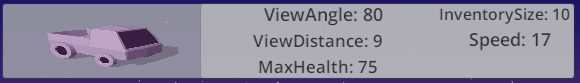
\includegraphics[scale=1]{StatsModel}
	\caption{Informations sur l'unité}
\end{figure}

\begin{enumerate}[label=\Alph*)]
\item\textbf{Affichage des statistiques de l'unité courante} \newline
Quand on choisit une unité, sur sa droite apparaît ses valeurs dans un cadre, cela correspond à ses statistiques. Cela va permettre à l'utilisateur d'adapter ses stratégies en fonction des statistiques de chaque unité.
Ces statistiques ne changent pas d'une équipe à l'autre, elles sont inhérentes à l'unité.
\item\textbf{Affichage du modèle 3D de l'unité courante} \newline
Dans le même cadre apparaît aussi le modèle 3D de l'unité courante. C'est l'apparence qu'aura l'unité en jeu.
\end{enumerate}


% Zone de création des comportements
\subsubsection{Liste des pièces}
\begin{enumerate}[label=\Alph*)]
\item\textbf{Boutons de choix de la catégorie de la pièce} \newline
Sur la gauche, de manière verticale, se trouve cinq noms de catégories qui sont les Contrôles, les Conditions, les Actions, les Messages et les Actions non terminales. En cliquant sur l'une de ces catégories, on affiche la liste des éléments de cette catégorie dans la zone directement à droite.
\item\textbf{Zone de sélection de la pièce suivant la catégorie} \newline
C'est dans cette zone qu’apparaît la liste des éléments des catégories de pièces de l'éditeur. La génération des modèles des pièces se fait de manière dynamique. Chaque type de pièce a un prefab associé. \newline
Un script contenant une méthode pour chaque type de pièces disponibles (Conditions, Actions, etc...), permet ce dynamisme. Voyons de plus près la gestion d'une des catégories de pièces (leur comportement est semblable).
\begin{itemize}
\item\textbf{UpdateCondition()} : Nous commençons par récupérer une structure UnitPerceptAction, contenant le nom d'une unité, ainsi que toutes les conditions, actions, et messages inhérents à l'unité.\newline
A partir de là, nous pouvons créer, à l'aide du prefab correspondant, une pièce, avec le label contenu dans notre structure.
Nous allons parcourir la structure pour créer toutes les pièces disponibles pour l'unité, et modifier leur placement, en leur ajoutant un vecteur, pour qu'elles ne se superposent pas.
\begin{lstlisting}[frame=single]
new Vector2(0, -button.GetComponent<RectTransform>().rect.height)+ deltaVect;
\end{lstlisting}
Dans cette fonction, nous nous occupons uniquement de la liste Conditions présente dans notre structure. Il y a une fonction pour chaque liste de la structure.

\item\textbf{createPuzzle.cs} : Lors de l'appel au script createPuzzle.cs, nous récupérons le prefab et le label associé au type de pièce concernée. Par exemple, pour une pièce "Conditions", nous récupérerons le prefab des pièces "Conditions", ainsi qu'un label nommé "PERCEPT". Le traitement de ce label se fait dans le script ConditionEditorScript.cs.\newline
Nous plaçons ensuite la pièce créée 

Lors d'un clic sur le modèle de pièce que l'on veut ajouter au comportement courant, la fonction create() est appelée. Une position par défaut est définie dans l'éditeur, qui déterminera où la pièce sera placée lors de sa création.\newline
A chaque pièce créée, nous l'ajoutons dans la liste listPieces, utilisée pour la fonction Annuler.

\begin{lstlisting}[frame=single]
puzzleClone.GetComponent<RectTransform>().anchoredPosition = new Vector3(positionInitial.x, positionInitial.y,15);
puzzleClone.transform.parent = GameObject.Find("Editeur").transform;
puzzleClone.GetComponent<RectTransform>().localPosition = new Vector3(puzzleClone.GetComponent<RectTransform>().localPosition.x, puzzleClone.GetComponent<RectTransform>().localPosition.y, 10);
\end{lstlisting}

Les pièces sont présentes sous forme de cases avec leur nom à l'intérieur (certaines possèdent des menus déroulant pour choisir la valeur voulue une fois dans la zone d'édition). La couleur des pièces dépend de leur catégorie.
Les pièces peuvent être sélectionnées et déplacées dans la zone d'édition du comportement grâce au glissé/déposé (Drag \& Drop).
\end{itemize}
\end{enumerate}

\subsubsection{Editeur}
C'est dans cette zone de l'éditeur que l’utilisateur pourra créer et modifier les comportements des untiés de ses équipes.
Nous voulions cette zone la plus grande possible, et la plus épurée possible, pour rendre le processus de création vraiment optimal.
\clearpage
\begin{figure}[h]
	\centering
		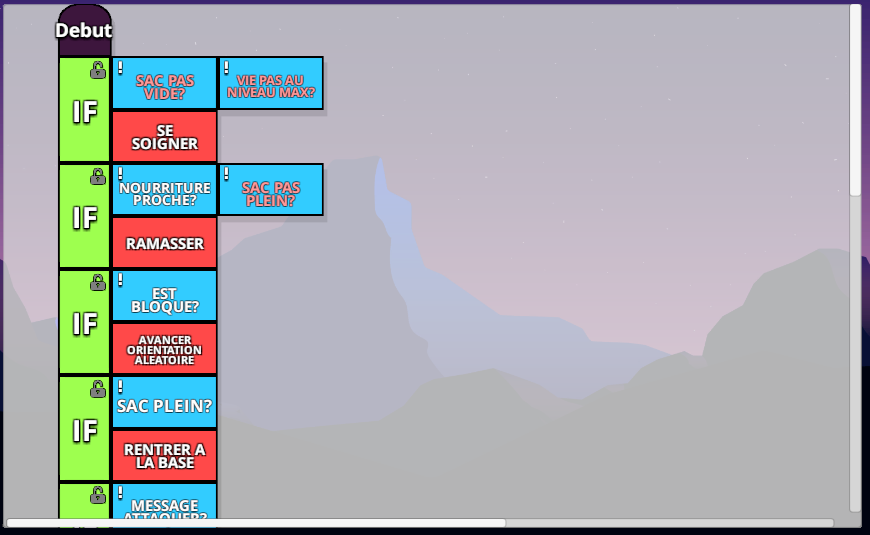
\includegraphics[scale=0.7]{ZoneEdition}
	\caption{Zone d'édition}
\end{figure}


\begin{enumerate}[label=\Alph*)]
\item\textbf{Zone éditeur de comportement de l'unité et de l'équipe courante} \newline
Dans cette zone arrivent les pièces venant de la zone de sélection. Elles se placent à l'aide du curseur de la souris sur une grille invisible. Si une pièce est valide, alors elle est colorée, sinon, elle est grise. Les pièces "IF" possèdent un cadenas dans le coin supérieur droit. Il permet de déplacer, en plus de la pièce IF, tout les éléments valides qui lui sont rattachés (hors IF). Les pièces de contrôles sont considérées comme valides si elles sont placées en dessous d'autres pièces du même type ou en dessous de la pièce "Start".\newline
Les autres pièces doivent se rattacher à des pièces de contrôle, en haut à droite pour les pièces Condition et en bas à droite pour les autres. Les pièces hors Contrôle sont ainsi valides lorsqu'elles sont au bon endroit, sur leur ligne, adjacentes au contrôle, ou adjacentes à une autre pièce du même type, valide. \newline \smallbreak

Voyons les scripts permettant cette gestion.

\begin{itemize}
\item\textbf{ManageDrapAndDrop.cs} : \newline 
Ce script s'occupe de la gestion du déplacement des pièces, ainsi que de leur placement, sur une grille aimantée.
\begin{itemize}
\item\textbf{OnMouseDrag()} : \newline
Une fois qu'un clic a été fait sur une pièce, cette fonction s'occupe de mettre à jour les coordonnées de la pièce, de telle sorte qu'elles soient égales à celles du pointeur de la souris. Pour valider les nouvelles coordonnées de la pièce, il faut appeler la fonction OnMouseUp().
\item\textbf{UpgradeGridPosition()} : \newline
Lorsque le clic de la souris est relâché (OnMouseUp), il faut mettre à jour la position de la pièce dans l'éditeur.
\begin{lstlisting}[frame=single]
posGridX = Mathf.Max((int)GameObject.Find("Editeur").GetComponent<RectTransform>().rect.x / 
  (int)widthPuzzle, (int)Mathf.Round(GetComponent<RectTransform>().localPosition.x / widthPuzzle));

posGridY = Mathf.Max((int)GameObject.Find("Editeur").GetComponent<RectTransform>().rect.y / 
  (int)heightPuzzle, (int)Mathf.Round(GetComponent<RectTransform>().localPosition.y / heightPuzzle));
\end{lstlisting}
\item\textbf{OnMouseUp()} : \newline
Cette fonction appelle la fonction UpdateGridPosition(), puis attribue à la pièce courante sa nouvelle position. Une fois cela fait, il faut vérifier que la nouvelle position de la pièce est toujours un emplacement valide, d'un point de vue comportement. La fonction appelle pour ça le script StartPuzzleScript.cs, que nous verrons plus bas.
\end{itemize}
\item\textbf{StartPuzzleScript.cs} : \newline
Ce script va nous permettre de vérifier si une pièce "If" est bien placée en dessous de la pièce Start.

\begin{itemize}
\item\textbf{UpdateAllValidPuzzles()} : \newline
Cette fonction, appelée dans ManageDragAndDrop.OnMouseUp(), va nous servir à vérifier si la position de la pièce "If" est correcte. Pour commencer, nous passons la variable booléenne "isValid" de toutes les pièces à false, puis nous allons vérifier leur placement.\newline
Pour se faire, nous allons appeler la fonction UpdatePuzzle() du script IfPuzzleScript.cs.\newline
Ensuite, si la pièce Start a bel et bien une pièce "If" juste en dessous d'elle, alors on passe la valeur isValid du "If" à true.
\end{itemize}

\item\textbf{IfPuzzleScript.cs} : \newline
Ce script s'occupe de vérifier le placement de toutes les pièces actuellement sur l'éditeur. Si leur positionnement n'est pas correct, leur couleur sera grise. Sinon, une pièce Contrôle sera verte, une pièce Condition sera bleue, une pièce Action Non Terminale sera orange, une pièce Action sera Rouge, et une pièce Message sera Jaune.
\begin{itemize}
\item\textbf{UpdateCondPuzzle()} : \newline
Cette fonction parcours toutes les pièces présentes sur l'éditeur. Si la pièce observée est une pièce de type Condition, et qu'elle est placée à droite d'une pièce "If", au niveau de sa première ligne, alors on l'attribue à une variable.

\begin{lstlisting}[frame=single]
if (currentGridPos + new Vector2(1,0) == puzzleGridPos && typePuzzle == PuzzleScript.Type.CONDITION)
\end{lstlisting}

\smallbreak
Cela nous permettra, dans UpdatePuzzle, de savoir que nous avons une pièce Condition placée à notre droite, sur la bonne ligne.
Le comportement des fonctions UpdateIfPuzzle() et UpdateActPuzzle est similaire. Le seul changement est la place dans l'éditeur. Une pièce "If" devra être située directement en dessous de notre "If" courant, et une pièce Action / Action non terminale / Message devra se trouver directement à droite de notre pièce "If", sur sa deuxième ligne.
\item\textbf{UpdatePuzzle()} : \newline
Cette fonction récupère les pièces adjacentes à notre pièce actuelle, à l'aide des scripts UpdateIfPuzzle(), UpdateCondPuzzle, UpdateActPuzzle(). Il met ensuite à jour les valeurs des pièces adjacentes, à savoir leur variable isValid, ainsi que leur variable NextPuzzle, qui leur permet de savoir quelle pièce leur est adjacente.

\end{itemize}
\end{itemize}
\end{enumerate}


\subsection{Écran de partie}
Pour l'écran en jeu, l'objectif était de conserver au maximum la lisibilité de l'action, tout en offrant l'accès à certaines options.
Nous affichons donc le nom des deux équipes participantes, de leur couleur correspondante. Dans la partie supérieure de l'écran, centré, nous pouvons apercevoir un compteur, indiquant la durée de la partie.

\begin{lstlisting}[language={[Sharp]C},label={lst:Update()}, caption= Extrait du code de TimerScriptHUD.cs]
timePassed += Time.deltaTime;
int mins = (int)(timePassed / 60);
int secs = (int)(timePassed % 60);
GetComponent<Text>().text = ("" + mins).PadLeft(2, '0') + ":" + ("" + secs).PadLeft(2, '0'); 
\end{lstlisting}	

Il y a également un diagramme circulaire, représentant la répartition des forces de chaque équipe. Au début de la partie, le diagramme est donc divisé en parts égales, en fonction du nombre d'équipes participantes. Cela nous permettra donc de suivre aisément le rapport de force entre chaque équipe.

\begin{lstlisting}[language={[Sharp]C},label={lst:Update()}, caption= Extrait du code de ScriptHUD.cs]
Dictionary<int, int> _score = new Dictionary<int, int>();
        
        for (int i = 0; i < GameObject.Find("GameManager").GetComponent<TeamManager>()._teams.Count; i ++)
        {
            _scores[i].color = GameObject.Find("GameManager").GetComponent<TeamManager>()._teams[i]._color;
            _scores[i].color = new Color(_scores[i].color.r, _scores[i].color.g, _scores[i].color.b, 1);
            _score[i] = 0;
        }
        float total = 0;
        foreach (GameObject unit in GameObject.FindGameObjectsWithTag("Unit"))
        {
            int teamUnit = unit.GetComponent<Stats>()._teamIndex;
            int scoreUnit = unit.GetComponent<Stats>().GetHealth();
            if (_score.ContainsKey(teamUnit))
            {
                _score[teamUnit] += scoreUnit;
            }
            else
            {
                _score[teamUnit] = scoreUnit;
            }
            total += scoreUnit;
        }
        float currentValue = 0;
        for (int i = 0; i < GameObject.Find("GameManager").GetComponent<TeamManager>()._teams.Count; i++)
        {
            currentValue += _score[i];
            _scores[i].fillAmount = currentValue / total;
        }
\end{lstlisting}	

D'autres éléments, que l'on pourrait diviser en trois parties, sont également présents sur cet écran.


\subsubsection{Caméras}
Dans le coin supérieur gauche de l'écran se trouvent deux boutons liés à la gestion des caméras.
Deux choix s'offrent à l'utilisateur : une caméra vue subjective, et la caméra par défaut.\\
La caméra subjective permet de placer une caméra sur une unité, et de voir à travers ses yeux. Pour activer cette caméra, il suffit de cliquer sur l'unité sur laquelle on désire se placer. On se retrouve donc sur notre unité. Avec les mouvements de la souris, on peut déplacer l'orientation de la caméra, nous permettant donc de scruter ce qu'il se passe autour de l'unité.
Cet affichage nous permet également de voir apparaître une fenêtre, regroupant la vie de l’unité, la contenance de son sac, et son orientation.
Pour quitter cette caméra, il suffit de cliquer à nouveau sur le bouton "FPS", qui remettra la caméra par défaut.

L'autre caméra offerte, accessible via le bouton "Libre", permet d'arrêter les déplacements de la caméra, pour avoir une caméra fixe, englobant tout le champ de bataille.

\subsubsection{Contrôles}
Dans le coin inférieur gauche de l'écran se trouvent deux boutons, et un nombre.
Les deux boutons permettent, au choix, de relancer la partie en cours, ou alors de la quitter, pour retourner au menu principal.\\
Pour relancer la partie en cours, il suffit de recharger la scène.

\begin{lstlisting}[language={[Sharp]C},label={lst:RestartScene()}, caption= Extrait du code de CanvasHUD.cs]
SceneManager.LoadScene(SceneManager.GetActiveScene().name);
\end{lstlisting}	

Le nombre que l'on voit représente le nombre d'images par secondes affichées.

\begin{lstlisting}[language={[Sharp]C},label={lst:Update()}, caption= Extrait du code de FPSScript.cs]
deltaTime += (Time.unscaledDeltaTime - deltaTime) * 0.1f;
float msec = deltaTime * 1000.0f;
float fps = 1.0f / deltaTime;
GetComponent<Text>().text = fps.ToString("00");
\end{lstlisting}	
 
\subsubsection{Gestion de partie}
Dans le coin inférieur droit se trouvent trois boutons, ainsi que deux sliders.
Chacun offre la possibilité de personnaliser l'affichage de la partie en cours, dynamiquement, ou de modifier des options.
\begin{enumerate}
\item\textbf{Statistiques}
Cliquer sur ce bouton active ou désactive l'affichage des points de vie des unités présentes en jeu. Cela nous permet de basculer entre un affichage détaillé, pour bien voir l'évolution des batailles, et l'état de santé d'une unité, à un affichage plus épuré, qui nous permet de profiter de l'action.\newline
Les barres de vie voient leur couleur modifiée en fonction de leur valeur. Cette couleur peut varier du vert, au rouge, en passant par l'orange.

\item\textbf{Messages}
Ce bouton nous permet d'activer / désactiver l'affichage de l'envoi de messages. A chaque message envoyé, un trait sera tracé, représentant la liaison entre l'émetteur et le récepteur. Cette option permet de suivre la communication entre les unités, au sein d'une équipe.

\item\textbf{Vision}
Ce bouton nous offre la possibilité d'afficher ou non le champ de vision de chaque unité. Cette option est très utile pour vérifier le comportement de chaque unité.\newline
En revanche, si l'on veut juste profiter du spectacle, il parait plus confortable de la désactiver, pour garder l'affichage épuré.

\begin{figure}[h]
	\centering
		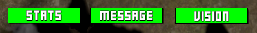
\includegraphics[scale=1]{OptionButtons}
	\caption{Boutons d'affichage, en jeu}
\end{figure}

\item\textbf{Vitesse de jeu}
Le slider placé au dessus des autres éléments de cette partie représente la vitesse à laquelle le temps défile. En modifiant sa valeur, le temps ralentit ou accélère, dynamiquement. Cette option, à l'image des précédentes, est très utile pour observer le comportement d'une unité, ou d'une équipe.
En revanche, si l'on veut connaître l'issu d'un combat rapidement, nous pouvons accélérer le temps.

\begin{figure}[h]
	\centering
		
\includegraphics[scale=1]{SpeedSlider}
	\caption{Barre de gestion de vitesse du jeu, en jeu}
\end{figure}

\item\textbf{Volume du jeu}
Le slider se trouvant juste en dessous du précédent permet, comme dans le menu des paramètres, de modifier le volume du son. L’icône sert de bouton; si on le presse, le son passe à 0 et l’icône devient barrée. Si l'on appuie de nouveau, il redevient classique, et le son est restitué à sa valeur précédente.
\end{enumerate}
\smallbreak
\begin{figure}[h]
	\centering
		
\includegraphics[scale=1]{ManuelJeu/SoundIG}
	\caption{Barre de son, en jeu}
\end{figure}

\section{Améliorations possibles}
Les fonctionnalités essentielles de l'interface on été mise en place, cependant, il reste beaucoup d'éléments 

qui aurait pu être implémentés avec plus de temps, ou de bugs qui auraient pu être résolus. Nous avons listé 

ces différents points :
\subsection{Fonctionnalités}
\begin{itemize}
\item InfoBulle apparaissant lors du passage du curseur au dessus d'un éléments de l'interface. 
\item Zone de comparaison de deux comportements à la fois, soit deux unités différentes soit la même unité mais 

dans deux équipes différentes.
\item ScrollBars dynamique dans la zone d'édition et dans la liste des pièces.
\item Bouton de sauvegarde qui change visuellement si le comportement courant n'est pas déjà sauvegardé.
\item Nouveau type de condition pour remplacer "Vie 75\%", "Vie 50\%", ... qui deviendrait une seule pièce avec 

un menu déroulant, qui contiendrait la liste des valeurs. 
\item Bruitage du jeu séparé de la musique du jeu. Dans l’intérêt que l'on puisse modifier l'un sans changer 

l'autre.
\item Une checkBox dans le menu des paramètres pour activer/désactiver le tir allié des unités.
\item Les boutons UNDO et REDO ne concerne que la création et la suppression des pièces de comportement. Une 

amélioration serait donc que ces boutons puisse aussi annuler le déplacement d'une pièce.
\item Bruitages en passant/appuyant sur les boutons (retour sonore).
\item Forme des pièces qui pourraient être de vraies pièce de puzzle, avec de vrais emboîtement visuels.
\item Animations visuelle des pièces lorsqu'elles sont au bon emplacement.
\item Animation et rotation des modèles 3D des unités.
\item Changement de l'aspect de l'éditeur suivant le jeu(fond d'écran, code couleur des pièces, musiques, 

etc...).
\item Image de présentation des cartes (Menu principal) qui tourne pour voir toute la carte.
\item Fenêtre de classement des équipes (score ELO).
\item Amélioration de la barre de chargement des parties qui est austère.
\item Bouton en jeu pour ouvrir l'éditeur de comportement sans arrêter la partie (et pouvoir modifier les 

comportements en direct).
\end{itemize}


\newpage
\part{L'avenir du projet}
\chapter{Pistes envisageables}
\paragraph{} Nous avons regroupé, dans ce chapitre, nos idées et nos pistes pour de possibles ajouts sur l'ensemble du projet.
\begin{itemize}
\item Implémenter de nouvelles maps
\item Ajouter de nouvelles unités au mode Warbot (Tourelles, Ingénieur et RocketLauncher)
\item Implémenter de nouveaux modes de jeux possédant leurs propres types d'unités, de comportement et d'élément de gameplay
\item Mettre en place la possibilité de sauvegarder une partie en cours, la quitter, et reprendre là où l'on s'était arrêté, en cliquant sur "Continuer partie"
\item Proposer un générateur de comportements aléatoires, configurable à l'aide de paramètres(équipe agressive, équipe défensive, etc...)
\item Possibilité de jouer en ligne
\item Partager ses équipes en ligne
\item Proposer un classement en ligne
\item Ajouter une liste de contacts
\item Ajouter un chat présent durant une partie
\item Proposer des aspects d'unités différents
\item Mettre en place des macros, avec niveau de complexité (débutant, avancé, confirmé, etc...), et proposer à l'utilisateur de pouvoir créer ses propres macros
\item Ajout de décor impactant le gameplay (untié qui se cache dans un buisson, une forêt)
\item Ajouter un mode debug en jeu
\end{itemize}

\chapter{Bugs}
Ce chapitre réunit les bugs connus dans notre projet.
\begin{enumerate}
\item\textbf{Scrollbar éditeur}\newline
La scrollbar de la zone d'édition du comportement n’est pas affectée par la molette de la souris. Seul celle des primitives l’est.
Si on rendait ça possible, le déplacement d'une pièce affectait les scrollbars, ce qui était un problème majeur.

\item\textbf{Undo / Redo}\newline
Si l'on annule une ou plusieurs créations / suppressions de pièces dans le comportement d'une unité, que l'on change d'unité, ou d'équipe, et qu'on clique sur "Redo", les pièces apparaîssent sur le comportement de la nouvelle unité.

\item\textbf{Suppression d'une équipe}\newline
Supprimer une équipe dans l’éditeur alors qu’il n’existe qu’un seule équipe ne fait pas disparaître la sous-fenêtre de confirmation de la suppression.
Pour faire disparaître la fenêtre, il faudra alors appuyer sur le bouton "Non".

\item\textbf{Placement de condition sur IF verrouillé}\newline
Quand on essaye de placer une condition à côté d'un IF qui est verrouillé, alors la condition ira par dessus le IF et non au bon endroit.

\item\textbf{Bug de collision des unités}\newline
Il arrive parfois que les unités sortent des limites de la zone de jeu et partent hors de portée de la caméra.
\end{enumerate}

\newpage
\part{Annexe}
\chapter{Scripts Remarquables}


\newpage
\section{ObjectPool.cs}
\lstinputlisting[language={[Sharp]C},label={lst:ObjectPoolScript}, caption=ObjectPool.cs]{ObjectPool.cs}
\newpage

\section{MovableCharacter.cs}
\lstinputlisting[language={[Sharp]C},label={lst:MovableCharacterScript}, caption=MovableCharacter.cs]{MovableCharacter.cs}
\newpage

\section{Brain.cs}
\lstinputlisting[language={[Sharp]C},label={lst:BrainScript}, caption=Brain.cs]{Brain.cs}
\newpage

\section{PerceptUnit.cs}
\lstinputlisting[language={[Sharp]C},label={lst:PerceptUnit}, caption=PerceptUnit.cs]{PerceptUnit.cs}
\newpage

\section{LoadFile.cs}
\lstinputlisting[language={[Sharp]C},label={lst:LoadFile}, caption=LoadFile.cs]{LoadFile.cs}
\newpage


\section{Stats.cs}
\lstinputlisting[language={[Sharp]C},label={lst:LoadFile}, caption=Stats.cs]{Stats.cs}
\newpage

\chapter{Image du jeu.}
\newpage
\begin{figure}[h]
	\centering
		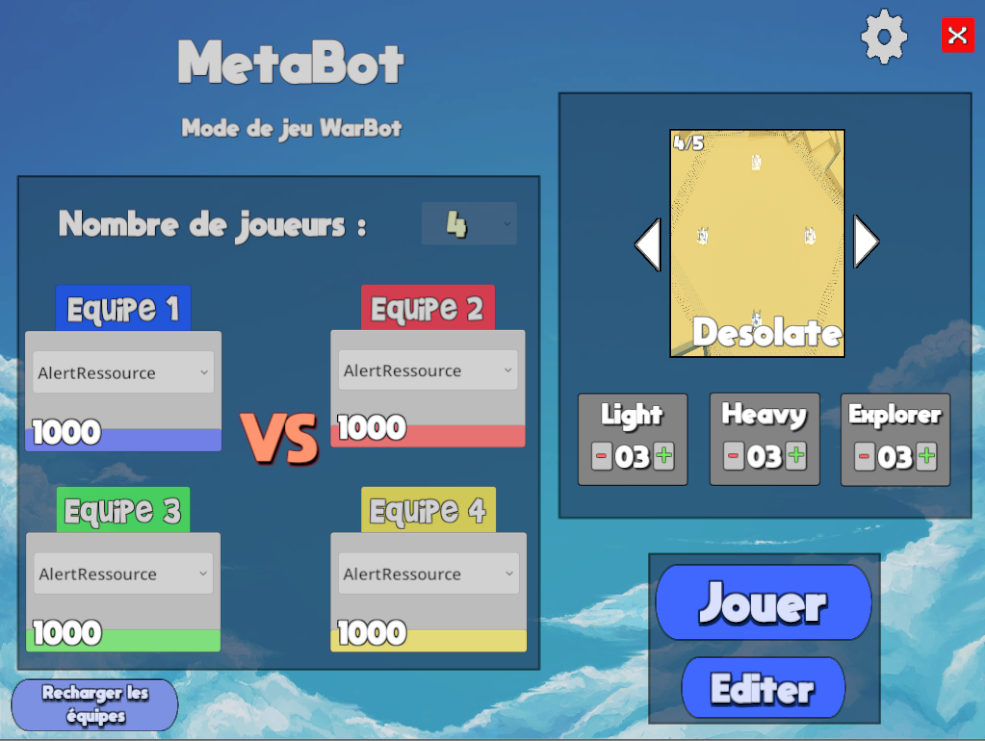
\includegraphics[scale=0.6]{MainMenuFrancais}
	\caption{Menu principal en français}
\end{figure}

\begin{figure}[h]
	\centering
		\includegraphics[scale=0.6]{MainMenuAnglais}
	\caption{Menu principal en anglais}
\end{figure}

\begin{figure}[h]
	\centering
		\includegraphics[scale=0.5]{PlainDemo}
	\caption{Partie du la carte Plain}
\end{figure}

\begin{figure}[h]
	\centering
		\includegraphics[scale=0.5]{DesolateDemo}
	\caption{Partie sur la carte Desolate}
\end{figure}

\begin{figure}[h]
	\centering
		\includegraphics[scale=0.5]{SimpleDemo}
	\caption{Partie sur la carte de Simple}
\end{figure}

\begin{figure}[h]
	\centering
		\includegraphics[scale=0.4]{Montagne}
	\caption{Partie sur la carte Mountain}
\end{figure}

\begin{figure}[h]
	\centering
		\includegraphics[scale=0.4]{Garden}
	\caption{Partie sur la carte Garden}
\end{figure}

% Uncomment the following two lines if you want to have a bibliography
%\bibliographystyle{alpha}
%\bibliography{document}

\end{document}

